\documentclass[10pt]{article}
\usepackage[letterpaper,margin=0.75in,top=0.8in,bottom=0.75in]{geometry}
\usepackage[T1]{fontenc}
\usepackage{lmodern}
\usepackage{microtype}
\usepackage{amsmath,amssymb,amsthm,bm}
\usepackage{booktabs,graphicx,xcolor,enumitem,caption,fancyhdr,titlesec,multicol,array}
\linespread{0.97}
\usepackage[ruled,vlined,linesnumbered]{algorithm2e}
\usepackage[colorlinks=true,linkcolor=blue!50!black,citecolor=blue!50!black,urlcolor=blue!50!black]{hyperref}

% Every number in this report is a macro written by experiments/make_figures.py from the files in results/.
% AUTO-GENERATED by experiments/make_figures.py from results/*.json -- do not edit by hand.
\newcommand{\AgreeEpsEoneBar}{86}
\newcommand{\AgreeEpsEoneSeats}{71}
\newcommand{\AgreeEpsEtwoBar}{86}
\newcommand{\AgreeEpsEtwoSeats}{72}
\newcommand{\AgreeEpsEzeroBar}{74}
\newcommand{\AgreeEpsEzeroSeats}{82}
\newcommand{\AgreeExpEoneBar}{94}
\newcommand{\AgreeExpEoneSeats}{81}
\newcommand{\AgreeExpEtwoBar}{93}
\newcommand{\AgreeExpEtwoSeats}{84}
\newcommand{\AgreeExpEzeroBar}{51}
\newcommand{\AgreeExpEzeroSeats}{93}
\newcommand{\AgreeEzeroBarMax}{74}
\newcommand{\AgreeEzeroBarMin}{51}
\newcommand{\AgreeMbEoneBar}{100}
\newcommand{\AgreeMbEoneSeats}{100}
\newcommand{\AgreeMbEtwoBar}{100}
\newcommand{\AgreeMbEtwoSeats}{100}
\newcommand{\AgreeMbEzeroBar}{56}
\newcommand{\AgreeMbEzeroSeats}{96}
\newcommand{\AgreeMidEpsEoneBar}{71}
\newcommand{\AgreeMidEpsEoneSeats}{57}
\newcommand{\AgreeMidEpsEtwoBar}{72}
\newcommand{\AgreeMidEpsEtwoSeats}{59}
\newcommand{\AgreeMidEpsEzeroBar}{72}
\newcommand{\AgreeMidEpsEzeroSeats}{77}
\newcommand{\AgreeMidExpEoneBar}{79}
\newcommand{\AgreeMidExpEoneSeats}{61}
\newcommand{\AgreeMidExpEtwoBar}{78}
\newcommand{\AgreeMidExpEtwoSeats}{61}
\newcommand{\AgreeMidExpEzeroBar}{55}
\newcommand{\AgreeMidExpEzeroSeats}{81}
\newcommand{\AgreeMidMbEoneBar}{99}
\newcommand{\AgreeMidMbEoneSeats}{93}
\newcommand{\AgreeMidMbEtwoBar}{99}
\newcommand{\AgreeMidMbEtwoSeats}{93}
\newcommand{\AgreeMidMbEzeroBar}{54}
\newcommand{\AgreeMidMbEzeroSeats}{91}
\newcommand{\AgreeMidMuEoneBar}{100}
\newcommand{\AgreeMidMuEoneSeats}{98}
\newcommand{\AgreeMidMuEtwoBar}{100}
\newcommand{\AgreeMidMuEtwoSeats}{96}
\newcommand{\AgreeMidMuEzeroBar}{52}
\newcommand{\AgreeMidMuEzeroSeats}{90}
\newcommand{\AgreeMidTsEoneBar}{92}
\newcommand{\AgreeMidTsEoneSeats}{71}
\newcommand{\AgreeMidTsEtwoBar}{91}
\newcommand{\AgreeMidTsEtwoSeats}{67}
\newcommand{\AgreeMidTsEzeroBar}{61}
\newcommand{\AgreeMidTsEzeroSeats}{92}
\newcommand{\AgreeMidUcbEoneBar}{93}
\newcommand{\AgreeMidUcbEoneSeats}{82}
\newcommand{\AgreeMidUcbEtwoBar}{95}
\newcommand{\AgreeMidUcbEtwoSeats}{80}
\newcommand{\AgreeMidUcbEzeroBar}{54}
\newcommand{\AgreeMidUcbEzeroSeats}{91}
\newcommand{\AgreeMuEoneBar}{100}
\newcommand{\AgreeMuEoneSeats}{100}
\newcommand{\AgreeMuEtwoBar}{100}
\newcommand{\AgreeMuEtwoSeats}{100}
\newcommand{\AgreeMuEzeroBar}{53}
\newcommand{\AgreeMuEzeroSeats}{96}
\newcommand{\AgreePooledEps}{78}
\newcommand{\AgreePooledExp}{83}
\newcommand{\AgreePooledMb}{92}
\newcommand{\AgreePooledMu}{92}
\newcommand{\AgreePooledTs}{91}
\newcommand{\AgreePooledUcb}{90}
\newcommand{\AgreeTsEoneBar}{99}
\newcommand{\AgreeTsEoneSeats}{92}
\newcommand{\AgreeTsEtwoBar}{99}
\newcommand{\AgreeTsEtwoSeats}{94}
\newcommand{\AgreeTsEzeroBar}{70}
\newcommand{\AgreeTsEzeroSeats}{93}
\newcommand{\AgreeUcbEoneBar}{99}
\newcommand{\AgreeUcbEoneSeats}{93}
\newcommand{\AgreeUcbEtwoBar}{99}
\newcommand{\AgreeUcbEtwoSeats}{94}
\newcommand{\AgreeUcbEzeroBar}{56}
\newcommand{\AgreeUcbEzeroSeats}{96}
\newcommand{\AstarGridBarAvg}{0.025}
\newcommand{\AstarGridBarStrong}{0.025}
\newcommand{\AstarGridBarWeak}{0.025}
\newcommand{\AstarGridSeatsAvg}{0.325--0.35}
\newcommand{\AstarGridSeatsStrong}{0.375--0.4}
\newcommand{\AstarGridSeatsWeak}{0.125}
\newcommand{\AstarLocalBarAvg}{0.01}
\newcommand{\AstarLocalBarStrong}{0.01}
\newcommand{\AstarLocalBarWeak}{0.01}
\newcommand{\AstarLocalSeatsAvg}{0.32}
\newcommand{\AstarLocalSeatsStrong}{0.38}
\newcommand{\AstarLocalSeatsWeak}{0.10}
\newcommand{\BarSeatsHigher}{12}
\newcommand{\BarSeatsNotSigLearners}{Leak-aware UCB, Model-based UCB}
\newcommand{\BarSeatsSig}{8}
\newcommand{\BarSeatsTests}{12}
\newcommand{\CceExHi}{99}
\newcommand{\CceExLo}{66}
\newcommand{\CceExN}{4}
\newcommand{\CceExPure}{67}
\newcommand{\CceMaxWidth}{0.417}
\newcommand{\CceMaxWidthEone}{0}
\newcommand{\CceMaxWidthEtwo}{0}
\newcommand{\CceMaxWidthEzero}{42}
\newcommand{\CceSingle}{267}
\newcommand{\CceSingleEone}{106}
\newcommand{\CceSingleEtwo}{106}
\newcommand{\CceSingleEzero}{55}
\newcommand{\CceTot}{318}
\newcommand{\CceTotEone}{106}
\newcommand{\CceTotEtwo}{106}
\newcommand{\CceTotEzero}{106}
\newcommand{\CceWiderEone}{0}
\newcommand{\CceWiderEtwo}{0}
\newcommand{\CceWiderEzero}{48}
\newcommand{\ChkDevPos}{0}
\newcommand{\ChkDevTot}{684}
\newcommand{\ChkDiya}{0.7088}
\newcommand{\ChkKabir}{0.7085}
\newcommand{\ChkOvertake}{0.9157}
\newcommand{\ChkPropThreeWorst}{2.2}
\newcommand{\ChkSpread}{0.29}
\newcommand{\ClanAlphaEffFull}{0.41}
\newcommand{\ClanBetaFull}{0.35}
\newcommand{\ClanMonotoneBar}{yes}
\newcommand{\ClanMonotoneSeats}{yes}
\newcommand{\ClanShareMaxBar}{100}
\newcommand{\ClanShareMaxSeats}{100}
\newcommand{\ClanShareMinBar}{100}
\newcommand{\ClanShareMinSeats}{33}
\newcommand{\CompBarAllShare}{19}
\newcommand{\CompGrid}{21}
\newcommand{\CompGridPos}{20}
\newcommand{\CompSeatsAllShare}{0}
\newcommand{\CompSeatsNoShare}{21}
\newcommand{\CrossQBarBetterFrom}{9}
\newcommand{\CrossQBarWorseUpTo}{6}
\newcommand{\DomOpenOutsideEzero}{1}
\newcommand{\DomOpenWhere}{two friend groups, E1, fixed seats, $\alpha=0.1$}
\newcommand{\DomPairsEoneSolved}{42}
\newcommand{\DomPairsEoneTot}{42}
\newcommand{\DomPairsEtwoSolved}{42}
\newcommand{\DomPairsEtwoTot}{42}
\newcommand{\DomPairsEzeroSolved}{39}
\newcommand{\DomPairsEzeroTot}{42}
\newcommand{\DomPairsSolved}{123}
\newcommand{\DomPairsTot}{126}
\newcommand{\DomSolved}{311}
\newcommand{\DomStarEoneSolved}{42}
\newcommand{\DomStarEoneTot}{42}
\newcommand{\DomStarEtwoSolved}{42}
\newcommand{\DomStarEtwoTot}{42}
\newcommand{\DomStarEzeroSolved}{12}
\newcommand{\DomStarEzeroTot}{42}
\newcommand{\DomStarSolved}{96}
\newcommand{\DomStarTot}{126}
\newcommand{\DomTot}{378}
\newcommand{\DomTwoGroupsEoneSolved}{41}
\newcommand{\DomTwoGroupsEoneTot}{42}
\newcommand{\DomTwoGroupsEtwoSolved}{42}
\newcommand{\DomTwoGroupsEtwoTot}{42}
\newcommand{\DomTwoGroupsEzeroSolved}{9}
\newcommand{\DomTwoGroupsEzeroTot}{42}
\newcommand{\DomTwoGroupsSolved}{92}
\newcommand{\DomTwoGroupsTot}{126}
\newcommand{\EllBarAvg}{0.00}
\newcommand{\EllBarStrong}{0.00}
\newcommand{\EllBarWeak}{0.00}
\newcommand{\EllSeatsAvg}{1.49}
\newcommand{\EllSeatsStrong}{1.60}
\newcommand{\EllSeatsWeak}{0.38}
\newcommand{\EpsBneEzero}{62}
\newcommand{\EpsBneGames}{378}
\newcommand{\EpsBneHeadBar}{1}
\newcommand{\EpsBneHeadSeats}{1}
\newcommand{\EpsBneLowAlpha}{17}
\newcommand{\EpsBneMulti}{117}
\newcommand{\EpsBneStep}{38}
\newcommand{\EpsBneStepMax}{64}
\newcommand{\ExactEqEpsEoneBar}{3}
\newcommand{\ExactEqEpsEoneSeats}{0}
\newcommand{\ExactEqEpsEtwoBar}{10}
\newcommand{\ExactEqEpsEtwoSeats}{0}
\newcommand{\ExactEqEpsEzeroBar}{0}
\newcommand{\ExactEqEpsEzeroSeats}{13}
\newcommand{\ExactEqExpEoneBar}{30}
\newcommand{\ExactEqExpEoneSeats}{3}
\newcommand{\ExactEqExpEtwoBar}{30}
\newcommand{\ExactEqExpEtwoSeats}{3}
\newcommand{\ExactEqExpEzeroBar}{0}
\newcommand{\ExactEqExpEzeroSeats}{20}
\newcommand{\ExactEqMbEoneBar}{100}
\newcommand{\ExactEqMbEoneSeats}{97}
\newcommand{\ExactEqMbEtwoBar}{100}
\newcommand{\ExactEqMbEtwoSeats}{100}
\newcommand{\ExactEqMbEzeroBar}{0}
\newcommand{\ExactEqMbEzeroSeats}{70}
\newcommand{\ExactEqMuEoneBar}{100}
\newcommand{\ExactEqMuEoneSeats}{100}
\newcommand{\ExactEqMuEtwoBar}{100}
\newcommand{\ExactEqMuEtwoSeats}{93}
\newcommand{\ExactEqMuEzeroBar}{0}
\newcommand{\ExactEqMuEzeroSeats}{63}
\newcommand{\ExactEqTsEoneBar}{87}
\newcommand{\ExactEqTsEoneSeats}{33}
\newcommand{\ExactEqTsEtwoBar}{83}
\newcommand{\ExactEqTsEtwoSeats}{27}
\newcommand{\ExactEqTsEzeroBar}{0}
\newcommand{\ExactEqTsEzeroSeats}{37}
\newcommand{\ExactEqUcbEoneBar}{87}
\newcommand{\ExactEqUcbEoneSeats}{40}
\newcommand{\ExactEqUcbEtwoBar}{93}
\newcommand{\ExactEqUcbEtwoSeats}{50}
\newcommand{\ExactEqUcbEzeroBar}{0}
\newcommand{\ExactEqUcbEzeroSeats}{70}
\newcommand{\ExplEpsEoneBar}{1.10}
\newcommand{\ExplEpsEoneSeats}{0.80}
\newcommand{\ExplEpsEtwoBar}{1.03}
\newcommand{\ExplEpsEtwoSeats}{0.79}
\newcommand{\ExplEpsEzeroBar}{0.10}
\newcommand{\ExplEpsEzeroSeats}{1.25}
\newcommand{\ExplExpEoneBar}{0.81}
\newcommand{\ExplExpEoneSeats}{0.75}
\newcommand{\ExplExpEtwoBar}{0.79}
\newcommand{\ExplExpEtwoSeats}{0.77}
\newcommand{\ExplExpEzeroBar}{0.10}
\newcommand{\ExplExpEzeroSeats}{0.66}
\newcommand{\ExplEzeroBarMax}{0.10}
\newcommand{\ExplEzeroBarMin}{0.10}
\newcommand{\ExplMbEoneBar}{0.00}
\newcommand{\ExplMbEoneSeats}{0.02}
\newcommand{\ExplMbEtwoBar}{0.00}
\newcommand{\ExplMbEtwoSeats}{0.00}
\newcommand{\ExplMbEzeroBar}{0.10}
\newcommand{\ExplMbEzeroSeats}{0.17}
\newcommand{\ExplMuEoneBar}{0.00}
\newcommand{\ExplMuEoneSeats}{0.00}
\newcommand{\ExplMuEtwoBar}{0.00}
\newcommand{\ExplMuEtwoSeats}{0.04}
\newcommand{\ExplMuEzeroBar}{0.10}
\newcommand{\ExplMuEzeroSeats}{0.27}
\newcommand{\ExplTsEoneBar}{0.14}
\newcommand{\ExplTsEoneSeats}{0.42}
\newcommand{\ExplTsEtwoBar}{0.16}
\newcommand{\ExplTsEtwoSeats}{0.48}
\newcommand{\ExplTsEzeroBar}{0.10}
\newcommand{\ExplTsEzeroSeats}{0.33}
\newcommand{\ExplUcbEoneBar}{0.14}
\newcommand{\ExplUcbEoneSeats}{0.36}
\newcommand{\ExplUcbEtwoBar}{0.07}
\newcommand{\ExplUcbEtwoSeats}{0.31}
\newcommand{\ExplUcbEzeroBar}{0.10}
\newcommand{\ExplUcbEzeroSeats}{0.17}
\newcommand{\GainBarAvg}{6.7}
\newcommand{\GainBarStrong}{6.7}
\newcommand{\GainBarWeak}{6.7}
\newcommand{\GainSeatsAvg}{4.9}
\newcommand{\GainSeatsStrong}{4.5}
\newcommand{\GainSeatsWeak}{4.5}
\newcommand{\GapEpsEoneBar}{0.51}
\newcommand{\GapEpsEoneSeats}{0.44}
\newcommand{\GapEpsEtwoBar}{0.51}
\newcommand{\GapEpsEtwoSeats}{0.42}
\newcommand{\GapEpsEzeroBar}{0.21}
\newcommand{\GapEpsEzeroSeats}{0.48}
\newcommand{\GapExpEoneBar}{0.94}
\newcommand{\GapExpEoneSeats}{0.54}
\newcommand{\GapExpEtwoBar}{0.93}
\newcommand{\GapExpEtwoSeats}{0.52}
\newcommand{\GapExpEzeroBar}{1.55}
\newcommand{\GapExpEzeroSeats}{1.15}
\newcommand{\GapFallSig}{6}
\newcommand{\GapFallTests}{6}
\newcommand{\GapFinalEps}{0.43}
\newcommand{\GapFinalExp}{0.94}
\newcommand{\GapFinalMax}{0.94}
\newcommand{\GapFinalMb}{0.60}
\newcommand{\GapFinalMin}{0.38}
\newcommand{\GapFinalMu}{0.44}
\newcommand{\GapFinalTs}{0.38}
\newcommand{\GapFinalUcb}{0.83}
\newcommand{\GapMbEoneBar}{0.16}
\newcommand{\GapMbEoneSeats}{0.52}
\newcommand{\GapMbEtwoBar}{0.24}
\newcommand{\GapMbEtwoSeats}{0.52}
\newcommand{\GapMbEzeroBar}{1.14}
\newcommand{\GapMbEzeroSeats}{1.01}
\newcommand{\GapMuEoneBar}{0.14}
\newcommand{\GapMuEoneSeats}{0.35}
\newcommand{\GapMuEtwoBar}{0.20}
\newcommand{\GapMuEtwoSeats}{0.37}
\newcommand{\GapMuEzeroBar}{0.83}
\newcommand{\GapMuEzeroSeats}{0.76}
\newcommand{\GapRatioEps}{0.52}
\newcommand{\GapRatioExp}{0.73}
\newcommand{\GapRatioMax}{0.73}
\newcommand{\GapRatioMb}{0.53}
\newcommand{\GapRatioMin}{0.42}
\newcommand{\GapRatioMu}{0.42}
\newcommand{\GapRatioTs}{0.45}
\newcommand{\GapRatioUcb}{0.73}
\newcommand{\GapTenKEps}{0.89}
\newcommand{\GapTenKExp}{1.67}
\newcommand{\GapTenKMb}{1.28}
\newcommand{\GapTenKMu}{1.17}
\newcommand{\GapTenKTs}{1.04}
\newcommand{\GapTenKUcb}{1.42}
\newcommand{\GapTsEoneBar}{0.46}
\newcommand{\GapTsEoneSeats}{0.39}
\newcommand{\GapTsEtwoBar}{0.48}
\newcommand{\GapTsEtwoSeats}{0.40}
\newcommand{\GapTsEzeroBar}{0.24}
\newcommand{\GapTsEzeroSeats}{0.33}
\newcommand{\GapUcbEoneBar}{0.90}
\newcommand{\GapUcbEoneSeats}{0.52}
\newcommand{\GapUcbEtwoBar}{0.91}
\newcommand{\GapUcbEtwoSeats}{0.52}
\newcommand{\GapUcbEzeroBar}{1.14}
\newcommand{\GapUcbEzeroSeats}{1.01}
\newcommand{\HtwoCells}{189}
\newcommand{\HtwoCellsNoEzero}{126}
\newcommand{\HtwoOk}{188}
\newcommand{\HtwoStrict}{134}
\newcommand{\HtwoViol}{1}
\newcommand{\HtwoViolBar}{67}
\newcommand{\HtwoViolBarN}{4}
\newcommand{\HtwoViolNoEzero}{0}
\newcommand{\HtwoViolSeatsHi}{78}
\newcommand{\HtwoViolSeatsLo}{61}
\newcommand{\HtwoViolSeatsN}{8}
\newcommand{\HtwoViolWhere}{two friend groups, E0, $\alpha=0.375$}
\newcommand{\LamAllBarQFifteen}{13.1}
\newcommand{\LamAllBarQFour}{57.6}
\newcommand{\LamAllRatioMax}{4.4}
\newcommand{\LamAllRatioMin}{2.5}
\newcommand{\LamAllSeatsQFifteen}{6.2}
\newcommand{\LamAllSeatsQFour}{17.6}
\newcommand{\LamBarQFifteen}{13.1}
\newcommand{\LamBarQFour}{57.6}
\newcommand{\LamBarQSixtyFour}{2.8}
\newcommand{\LamCIBarQFifteen}{13.1, 13.2}
\newcommand{\LamCIBarQFour}{57.5, 57.8}
\newcommand{\LamCIBarQSixtyFour}{2.7, 2.8}
\newcommand{\LamCISeatsQFifteen}{1.7, 1.7}
\newcommand{\LamCISeatsQFour}{9.1, 9.3}
\newcommand{\LamCISeatsQSixtyFour}{0.3, 0.4}
\newcommand{\LamOrderHolds}{11}
\newcommand{\LamOrderTot}{11}
\newcommand{\LamRatioMax}{12}
\newcommand{\LamRatioMin}{8}
\newcommand{\LamSeatsQFifteen}{1.7}
\newcommand{\LamSeatsQFour}{9.2}
\newcommand{\LamSeatsQSixtyFour}{0.3}
\newcommand{\MbEarlyEoneBar}{+12}
\newcommand{\MbEarlyEoneSeats}{+13}
\newcommand{\MbEarlyEtwoBar}{+7}
\newcommand{\MbEarlyEtwoSeats}{+11}
\newcommand{\MbEarlyEzeroBar}{+0}
\newcommand{\MbEarlyEzeroSeats}{+0}
\newcommand{\MbEarlyPEoneBar}{0.001}
\newcommand{\MbEarlyPEoneSeats}{0.020}
\newcommand{\MbEarlyPEtwoBar}{0.015}
\newcommand{\MbEarlyPEtwoSeats}{0.020}
\newcommand{\MbEarlyPEzeroBar}{1.000}
\newcommand{\MbEarlyPEzeroSeats}{1.000}
\newcommand{\MbEarlySig}{4}
\newcommand{\MbEarlyTests}{4}
\newcommand{\MbFinalEoneBar}{+1}
\newcommand{\MbFinalEoneSeats}{+7}
\newcommand{\MbFinalEtwoBar}{+1}
\newcommand{\MbFinalEtwoSeats}{+6}
\newcommand{\MbFinalEzeroBar}{+0}
\newcommand{\MbFinalEzeroSeats}{+0}
\newcommand{\MbFinalPEoneBar}{1.000}
\newcommand{\MbFinalPEoneSeats}{0.001}
\newcommand{\MbFinalPEtwoBar}{1.000}
\newcommand{\MbFinalPEtwoSeats}{0.002}
\newcommand{\MbFinalPEzeroBar}{1.000}
\newcommand{\MbFinalPEzeroSeats}{1.000}
\newcommand{\MbLeakHatEone}{0.200}
\newcommand{\MbLeakHatEtwo}{0.200}
\newcommand{\MbLeakHatEzero}{1.000}
\newcommand{\MbRegretEoneBar}{-351}
\newcommand{\MbRegretEoneSeats}{+2}
\newcommand{\MbRegretEtwoBar}{-322}
\newcommand{\MbRegretEtwoSeats}{+2}
\newcommand{\MbRegretEzeroBar}{+0}
\newcommand{\MbRegretEzeroSeats}{+0}
\newcommand{\MbRegretPEoneBar}{0.001}
\newcommand{\MbRegretPEoneSeats}{1.000}
\newcommand{\MbRegretPEtwoBar}{0.001}
\newcommand{\MbRegretPEtwoSeats}{1.000}
\newcommand{\MbRegretPEzeroBar}{1.000}
\newcommand{\MbRegretPEzeroSeats}{1.000}
\newcommand{\MbRegretSig}{2}
\newcommand{\MbRegretTests}{4}
\newcommand{\MbSameAsUcbEzero}{yes}
\newcommand{\MixedCells}{120}
\newcommand{\MixedDiffCells}{1}
\newcommand{\MixedGames}{10}
\newcommand{\MixedSameGames}{9}
\newcommand{\MuEarlyEoneBar}{+15}
\newcommand{\MuEarlyEoneSeats}{+24}
\newcommand{\MuEarlyEtwoBar}{+10}
\newcommand{\MuEarlyEtwoSeats}{+20}
\newcommand{\MuEarlyEzeroBar}{-1}
\newcommand{\MuEarlyEzeroSeats}{-3}
\newcommand{\MuEarlyPEoneBar}{0.001}
\newcommand{\MuEarlyPEoneSeats}{0.001}
\newcommand{\MuEarlyPEtwoBar}{0.001}
\newcommand{\MuEarlyPEtwoSeats}{0.001}
\newcommand{\MuEarlyPEzeroBar}{1.000}
\newcommand{\MuEarlyPEzeroSeats}{1.000}
\newcommand{\MuEarlySig}{4}
\newcommand{\MuEarlyTests}{4}
\newcommand{\MuFinalEoneBar}{+1}
\newcommand{\MuFinalEoneSeats}{+7}
\newcommand{\MuFinalEtwoBar}{+1}
\newcommand{\MuFinalEtwoSeats}{+6}
\newcommand{\MuFinalEzeroBar}{-3}
\newcommand{\MuFinalEzeroSeats}{-0}
\newcommand{\MuFinalPEoneBar}{1.000}
\newcommand{\MuFinalPEoneSeats}{0.001}
\newcommand{\MuFinalPEtwoBar}{1.000}
\newcommand{\MuFinalPEtwoSeats}{0.001}
\newcommand{\MuFinalPEzeroBar}{0.393}
\newcommand{\MuFinalPEzeroSeats}{1.000}
\newcommand{\MuLeakHatEone}{0.200}
\newcommand{\MuLeakHatEtwo}{0.200}
\newcommand{\MuLeakHatEzero}{1.000}
\newcommand{\MuRegretEoneBar}{-356}
\newcommand{\MuRegretEoneSeats}{-77}
\newcommand{\MuRegretEtwoBar}{-330}
\newcommand{\MuRegretEtwoSeats}{-67}
\newcommand{\MuRegretEzeroBar}{-96}
\newcommand{\MuRegretEzeroSeats}{-79}
\newcommand{\MuRegretPEoneBar}{0.001}
\newcommand{\MuRegretPEoneSeats}{0.001}
\newcommand{\MuRegretPEtwoBar}{0.001}
\newcommand{\MuRegretPEtwoSeats}{0.001}
\newcommand{\MuRegretPEzeroBar}{0.001}
\newcommand{\MuRegretPEzeroSeats}{0.001}
\newcommand{\MuRegretSig}{4}
\newcommand{\MuRegretTests}{4}
\newcommand{\NumEqEoneBar}{1}
\newcommand{\NumEqEoneSeats}{1}
\newcommand{\NumEqEtwoBar}{1}
\newcommand{\NumEqEtwoSeats}{1}
\newcommand{\NumEqEzeroBar}{4}
\newcommand{\NumEqEzeroSeats}{2}
\newcommand{\PayGapMaxEoneBar}{0.99}
\newcommand{\PayGapMaxEoneSeats}{0.80}
\newcommand{\PayGapMaxEtwoBar}{0.98}
\newcommand{\PayGapMaxEtwoSeats}{0.78}
\newcommand{\PayGapMaxEzeroBar}{6.62}
\newcommand{\PayGapMaxEzeroSeats}{2.79}
\newcommand{\PayGapMinEoneBar}{0.96}
\newcommand{\PayGapMinEoneSeats}{0.36}
\newcommand{\PayGapMinEtwoBar}{0.97}
\newcommand{\PayGapMinEtwoSeats}{0.36}
\newcommand{\PayGapMinEzeroBar}{0.10}
\newcommand{\PayGapMinEzeroSeats}{0.42}
\newcommand{\PayGapTypeEoneBarAvg}{0.98}
\newcommand{\PayGapTypeEoneBarStrong}{0.97}
\newcommand{\PayGapTypeEoneBarWeak}{0.98}
\newcommand{\PayGapTypeEoneSeatsAvg}{0.55}
\newcommand{\PayGapTypeEoneSeatsStrong}{0.76}
\newcommand{\PayGapTypeEoneSeatsWeak}{0.40}
\newcommand{\PayGapTypeEtwoBarAvg}{0.98}
\newcommand{\PayGapTypeEtwoBarStrong}{0.98}
\newcommand{\PayGapTypeEtwoBarWeak}{0.97}
\newcommand{\PayGapTypeEtwoSeatsAvg}{0.55}
\newcommand{\PayGapTypeEtwoSeatsStrong}{0.77}
\newcommand{\PayGapTypeEtwoSeatsWeak}{0.39}
\newcommand{\PayGapTypeEzeroBarAvg}{3.36}
\newcommand{\PayGapTypeEzeroBarStrong}{3.35}
\newcommand{\PayGapTypeEzeroBarWeak}{3.35}
\newcommand{\PayGapTypeEzeroSeatsAvg}{0.44}
\newcommand{\PayGapTypeEzeroSeatsStrong}{2.77}
\newcommand{\PayGapTypeEzeroSeatsWeak}{2.16}
\newcommand{\PilotBootFracBar}{100}
\newcommand{\PilotBootFracSeats}{100}
\newcommand{\PilotBootRBar}{200}
\newcommand{\PilotBootRSeats}{200}
\newcommand{\PilotShareBar}{100}
\newcommand{\PilotShareSeats}{33}
\newcommand{\QFiveAllBar}{40}
\newcommand{\QFiveAllSeats}{20}
\newcommand{\QFiveBar}{40}
\newcommand{\QFiveCIBar}{40}
\newcommand{\QFiveCISeats}{9}
\newcommand{\QFiveSeats}{9}
\newcommand{\RegretEpsEoneBar}{178}
\newcommand{\RegretEpsEoneSeats}{154}
\newcommand{\RegretEpsEtwoBar}{174}
\newcommand{\RegretEpsEtwoSeats}{147}
\newcommand{\RegretEpsEzeroBar}{81}
\newcommand{\RegretEpsEzeroSeats}{146}
\newcommand{\RegretExpEoneBar}{442}
\newcommand{\RegretExpEoneSeats}{251}
\newcommand{\RegretExpEtwoBar}{441}
\newcommand{\RegretExpEtwoSeats}{247}
\newcommand{\RegretExpEzeroBar}{706}
\newcommand{\RegretExpEzeroSeats}{512}
\newcommand{\RegretMbEoneBar}{70}
\newcommand{\RegretMbEoneSeats}{247}
\newcommand{\RegretMbEtwoBar}{98}
\newcommand{\RegretMbEtwoSeats}{247}
\newcommand{\RegretMbEzeroBar}{466}
\newcommand{\RegretMbEzeroSeats}{463}
\newcommand{\RegretMuEoneBar}{65}
\newcommand{\RegretMuEoneSeats}{168}
\newcommand{\RegretMuEtwoBar}{89}
\newcommand{\RegretMuEtwoSeats}{178}
\newcommand{\RegretMuEzeroBar}{370}
\newcommand{\RegretMuEzeroSeats}{384}
\newcommand{\RegretTsEoneBar}{191}
\newcommand{\RegretTsEoneSeats}{173}
\newcommand{\RegretTsEtwoBar}{197}
\newcommand{\RegretTsEtwoSeats}{179}
\newcommand{\RegretTsEzeroBar}{93}
\newcommand{\RegretTsEzeroSeats}{158}
\newcommand{\RegretUcbEoneBar}{421}
\newcommand{\RegretUcbEoneSeats}{246}
\newcommand{\RegretUcbEtwoBar}{420}
\newcommand{\RegretUcbEtwoSeats}{245}
\newcommand{\RegretUcbEzeroBar}{466}
\newcommand{\RegretUcbEzeroSeats}{463}
\newcommand{\SuppPairsComplete}{123}
\newcommand{\SuppPairsGames}{126}
\newcommand{\SuppPairsMaxFree}{3}
\newcommand{\SuppPairsMixedGames}{3}
\newcommand{\SuppPairsMixedTotal}{3}
\newcommand{\SuppPairsPureOk}{126}
\newcommand{\TninetyEpsEoneBar}{never}
\newcommand{\TninetyEpsEoneSeats}{never}
\newcommand{\TninetyEpsEtwoBar}{160{,}500}
\newcommand{\TninetyEpsEtwoSeats}{never}
\newcommand{\TninetyEpsEzeroBar}{never}
\newcommand{\TninetyEpsEzeroSeats}{never}
\newcommand{\TninetyExpEoneBar}{61{,}000}
\newcommand{\TninetyExpEoneSeats}{141{,}000}
\newcommand{\TninetyExpEtwoBar}{41{,}000}
\newcommand{\TninetyExpEtwoSeats}{122{,}000}
\newcommand{\TninetyExpEzeroBar}{never}
\newcommand{\TninetyExpEzeroSeats}{29{,}000}
\newcommand{\TninetyMbEoneBar}{7{,}000}
\newcommand{\TninetyMbEoneSeats}{27{,}000}
\newcommand{\TninetyMbEtwoBar}{8{,}500}
\newcommand{\TninetyMbEtwoSeats}{28{,}500}
\newcommand{\TninetyMbEzeroBar}{never}
\newcommand{\TninetyMbEzeroSeats}{16{,}500}
\newcommand{\TninetyMuEoneBar}{4{,}500}
\newcommand{\TninetyMuEoneSeats}{12{,}000}
\newcommand{\TninetyMuEtwoBar}{4{,}000}
\newcommand{\TninetyMuEtwoSeats}{15{,}500}
\newcommand{\TninetyMuEzeroBar}{never}
\newcommand{\TninetyMuEzeroSeats}{12{,}000}
\newcommand{\TninetyTsEoneBar}{19{,}000}
\newcommand{\TninetyTsEoneSeats}{78{,}000}
\newcommand{\TninetyTsEtwoBar}{16{,}500}
\newcommand{\TninetyTsEtwoSeats}{80{,}000}
\newcommand{\TninetyTsEzeroBar}{never}
\newcommand{\TninetyTsEzeroSeats}{19{,}500}
\newcommand{\TninetyUcbEoneBar}{18{,}000}
\newcommand{\TninetyUcbEoneSeats}{56{,}000}
\newcommand{\TninetyUcbEtwoBar}{12{,}000}
\newcommand{\TninetyUcbEtwoSeats}{60{,}500}
\newcommand{\TninetyUcbEzeroBar}{never}
\newcommand{\TninetyUcbEzeroSeats}{16{,}500}
\newcommand{\TypeEpsEoneBarAvg}{71}
\newcommand{\TypeEpsEoneBarStrong}{77}
\newcommand{\TypeEpsEoneBarWeak}{95}
\newcommand{\TypeEpsEoneSeatsAvg}{64}
\newcommand{\TypeEpsEoneSeatsStrong}{65}
\newcommand{\TypeEpsEoneSeatsWeak}{70}
\newcommand{\TypeEpsEtwoBarAvg}{75}
\newcommand{\TypeEpsEtwoBarStrong}{77}
\newcommand{\TypeEpsEtwoBarWeak}{92}
\newcommand{\TypeEpsEtwoSeatsAvg}{60}
\newcommand{\TypeEpsEtwoSeatsStrong}{72}
\newcommand{\TypeEpsEtwoSeatsWeak}{73}
\newcommand{\TypeEpsEzeroBarAvg}{75}
\newcommand{\TypeEpsEzeroBarStrong}{68}
\newcommand{\TypeEpsEzeroBarWeak}{73}
\newcommand{\TypeEpsEzeroSeatsAvg}{64}
\newcommand{\TypeEpsEzeroSeatsStrong}{82}
\newcommand{\TypeEpsEzeroSeatsWeak}{93}
\newcommand{\TypeExpEoneBarAvg}{93}
\newcommand{\TypeExpEoneBarStrong}{80}
\newcommand{\TypeExpEoneBarWeak}{100}
\newcommand{\TypeExpEoneSeatsAvg}{73}
\newcommand{\TypeExpEoneSeatsStrong}{73}
\newcommand{\TypeExpEoneSeatsWeak}{82}
\newcommand{\TypeExpEtwoBarAvg}{95}
\newcommand{\TypeExpEtwoBarStrong}{79}
\newcommand{\TypeExpEtwoBarWeak}{100}
\newcommand{\TypeExpEtwoSeatsAvg}{79}
\newcommand{\TypeExpEtwoSeatsStrong}{78}
\newcommand{\TypeExpEtwoSeatsWeak}{84}
\newcommand{\TypeExpEzeroBarAvg}{51}
\newcommand{\TypeExpEzeroBarStrong}{52}
\newcommand{\TypeExpEzeroBarWeak}{50}
\newcommand{\TypeExpEzeroSeatsAvg}{78}
\newcommand{\TypeExpEzeroSeatsStrong}{99}
\newcommand{\TypeExpEzeroSeatsWeak}{98}
\newcommand{\TypeMbEoneBarAvg}{100}
\newcommand{\TypeMbEoneBarStrong}{100}
\newcommand{\TypeMbEoneBarWeak}{100}
\newcommand{\TypeMbEoneSeatsAvg}{99}
\newcommand{\TypeMbEoneSeatsStrong}{100}
\newcommand{\TypeMbEoneSeatsWeak}{100}
\newcommand{\TypeMbEtwoBarAvg}{100}
\newcommand{\TypeMbEtwoBarStrong}{100}
\newcommand{\TypeMbEtwoBarWeak}{100}
\newcommand{\TypeMbEtwoSeatsAvg}{100}
\newcommand{\TypeMbEtwoSeatsStrong}{100}
\newcommand{\TypeMbEtwoSeatsWeak}{100}
\newcommand{\TypeMbEzeroBarAvg}{60}
\newcommand{\TypeMbEzeroBarStrong}{56}
\newcommand{\TypeMbEzeroBarWeak}{52}
\newcommand{\TypeMbEzeroSeatsAvg}{90}
\newcommand{\TypeMbEzeroSeatsStrong}{100}
\newcommand{\TypeMbEzeroSeatsWeak}{99}
\newcommand{\TypeMuEoneBarAvg}{100}
\newcommand{\TypeMuEoneBarStrong}{100}
\newcommand{\TypeMuEoneBarWeak}{100}
\newcommand{\TypeMuEoneSeatsAvg}{100}
\newcommand{\TypeMuEoneSeatsStrong}{100}
\newcommand{\TypeMuEoneSeatsWeak}{100}
\newcommand{\TypeMuEtwoBarAvg}{100}
\newcommand{\TypeMuEtwoBarStrong}{100}
\newcommand{\TypeMuEtwoBarWeak}{100}
\newcommand{\TypeMuEtwoSeatsAvg}{98}
\newcommand{\TypeMuEtwoSeatsStrong}{100}
\newcommand{\TypeMuEtwoSeatsWeak}{100}
\newcommand{\TypeMuEzeroBarAvg}{60}
\newcommand{\TypeMuEzeroBarStrong}{50}
\newcommand{\TypeMuEzeroBarWeak}{50}
\newcommand{\TypeMuEzeroSeatsAvg}{89}
\newcommand{\TypeMuEzeroSeatsStrong}{100}
\newcommand{\TypeMuEzeroSeatsWeak}{99}
\newcommand{\TypeTsEoneBarAvg}{98}
\newcommand{\TypeTsEoneBarStrong}{99}
\newcommand{\TypeTsEoneBarWeak}{100}
\newcommand{\TypeTsEoneSeatsAvg}{82}
\newcommand{\TypeTsEoneSeatsStrong}{92}
\newcommand{\TypeTsEoneSeatsWeak}{94}
\newcommand{\TypeTsEtwoBarAvg}{98}
\newcommand{\TypeTsEtwoBarStrong}{98}
\newcommand{\TypeTsEtwoBarWeak}{100}
\newcommand{\TypeTsEtwoSeatsAvg}{82}
\newcommand{\TypeTsEtwoSeatsStrong}{91}
\newcommand{\TypeTsEtwoSeatsWeak}{92}
\newcommand{\TypeTsEzeroBarAvg}{65}
\newcommand{\TypeTsEzeroBarStrong}{64}
\newcommand{\TypeTsEzeroBarWeak}{64}
\newcommand{\TypeTsEzeroSeatsAvg}{78}
\newcommand{\TypeTsEzeroSeatsStrong}{100}
\newcommand{\TypeTsEzeroSeatsWeak}{100}
\newcommand{\TypeUcbEoneBarAvg}{97}
\newcommand{\TypeUcbEoneBarStrong}{100}
\newcommand{\TypeUcbEoneBarWeak}{100}
\newcommand{\TypeUcbEoneSeatsAvg}{83}
\newcommand{\TypeUcbEoneSeatsStrong}{96}
\newcommand{\TypeUcbEoneSeatsWeak}{99}
\newcommand{\TypeUcbEtwoBarAvg}{99}
\newcommand{\TypeUcbEtwoBarStrong}{99}
\newcommand{\TypeUcbEtwoBarWeak}{100}
\newcommand{\TypeUcbEtwoSeatsAvg}{92}
\newcommand{\TypeUcbEtwoSeatsStrong}{95}
\newcommand{\TypeUcbEtwoSeatsWeak}{95}
\newcommand{\TypeUcbEzeroBarAvg}{60}
\newcommand{\TypeUcbEzeroBarStrong}{56}
\newcommand{\TypeUcbEzeroBarWeak}{52}
\newcommand{\TypeUcbEzeroSeatsAvg}{90}
\newcommand{\TypeUcbEzeroSeatsStrong}{100}
\newcommand{\TypeUcbEzeroSeatsWeak}{99}
\newcommand{\VEqBarQFifteen}{0.78}
\newcommand{\VEqBarQFour}{0.38}
\newcommand{\VEqSeatsQFifteen}{0.65}
\newcommand{\VEqSeatsQFour}{0.60}
\newcommand{\VNoLeakBar}{0.89}
\newcommand{\VNoLeakSeats}{0.66}
\newcommand{\XfourBarShareSame}{yes}
\newcommand{\XfourBoot}{500}
\newcommand{\XfourSeatsShareSame}{yes}
\newcommand{\XfourShareBar}{100}
\newcommand{\XfourShareSeats}{33}
\newcommand{\XoneBootOk}{370}
\newcommand{\XoneBootOkPct}{98}
\newcommand{\XoneBootTot}{378}
\newcommand{\XoneBrdOk}{3024}
\newcommand{\XoneBrdTot}{3024}
\newcommand{\XoneCells}{378}
\newcommand{\XoneMulti}{63}
\newcommand{\XoneMultiEnvs}{E0}
\newcommand{\XoneNone}{0}
\newcommand{\XoneRepMatch}{375}
\newcommand{\XoneRepRest}{3}
\newcommand{\XoneRepTot}{378}
\newcommand{\XoneUnique}{315}
\newcommand{\XoneWorstEps}{0.0003}
\newcommand{\XoneWorstEpsPP}{0.03}
\newcommand{\XthreeRuns}{1080}
\newcommand{\XthreeSeeds}{30}
\newcommand{\XthreeT}{200{,}000}
\newcommand{\XtwoMulti}{0}
\newcommand{\XtwoNoPure}{0}

\newcommand{\RepoURL}{https://github.com/Vish-Overflows/multiagent-systems-leak-or-keep}

% ---------- layout ----------
\pagestyle{fancy}\fancyhf{}
\fancyhead[L]{\small Leak or Keep? Learning to Share Interview Questions}
\fancyhead[R]{\small\scshape Final Project Report}
\fancyfoot[C]{\small\thepage}
\renewcommand{\headrulewidth}{0.4pt}
\titlespacing*{\section}{0pt}{6pt plus 2pt}{2.5pt}
\titlespacing*{\subsection}{0pt}{4pt plus 2pt}{1.5pt}
\titleformat{\section}{\normalfont\large\bfseries}{\thesection}{0.6em}{}
\titleformat{\subsection}{\normalfont\normalsize\bfseries}{\thesubsection}{0.6em}{}
\setlength{\parskip}{2pt plus 1pt}\setlength{\parindent}{0pt}
\setlist{nosep,leftmargin=1.3em,topsep=1pt}
\captionsetup{font=small,labelfont=bf,skip=3pt}
\setlength{\textfloatsep}{6pt plus 2pt}\setlength{\floatsep}{5pt plus 2pt}\setlength{\intextsep}{5pt plus 2pt}
\setlength{\abovedisplayskip}{3pt}\setlength{\belowdisplayskip}{3pt}
\SetAlFnt{\small}\SetAlCapFnt{\small}\SetAlCapNameFnt{\small}\setlength{\algomargin}{1.2em}
\renewcommand{\topfraction}{0.95}\renewcommand{\bottomfraction}{0.9}\renewcommand{\textfraction}{0.05}\renewcommand{\floatpagefraction}{0.9}
\setcounter{topnumber}{4}\setcounter{bottomnumber}{3}\setcounter{totalnumber}{6}

\theoremstyle{plain}
\newtheorem{lemma}{Lemma}\newtheorem{proposition}{Proposition}\newtheorem{corollary}{Corollary}
\theoremstyle{definition}\newtheorem{definition}{Definition}
\makeatletter\def\thm@space@setup{\thm@preskip=3pt \thm@postskip=2pt}\makeatother

\newcommand{\E}{\mathbb{E}}\newcommand{\1}{\mathbf{1}}
\newcommand{\seats}{\textsc{Seats}}\newcommand{\barr}{\textsc{Bar}}
\newcommand{\finding}[1]{\textbf{#1}}
\newcommand{\plain}[1]{\emph{#1}}

\begin{document}
\thispagestyle{plain}
\begin{center}
{\Large\bfseries\scshape Leak or Keep?\\[2pt] Learning to Share Interview Questions Among Competing Candidates}\\[5pt]
{\small\scshape Final Project Report --- Multi-Agent Systems, IIT Gandhinagar}\\[6pt]
{\small\setlength{\tabcolsep}{4pt}
\begin{tabular}{cccc}
\textbf{Jash Bharat Pasad} & \textbf{Bhavay Goyal} & \textbf{Chaitanya Bhoite} & \textbf{Vishnu Sinha}\\
24110146 & 24110070 & 24110086 & 24110389\\
\texttt{jash.pasad@iitgn.ac.in} & \texttt{bhavay.goyal@iitgn.ac.in} & \texttt{chaitanya.bhoite@iitgn.ac.in} & \texttt{vishnu.sinha@iitgn.ac.in}
\end{tabular}}\\[4pt]
{\small Code, result files and commands that regenerate every number below: \url{\RepoURL}}
\end{center}

\begin{center}\begin{minipage}{0.94\textwidth}\small
\textbf{\scshape Abstract.}
After an interview, a candidate can tell friends who interview later which questions were asked. This helps them, but they may be
competing for the same offers. We model this as a game on an $n\times n$ sharing matrix: candidates interview in a fixed order, know
only a coarse ability type (never their score), and a shared question may not reappear.
We solve the six-candidate game \emph{exactly} for \XoneCells{} combinations of hiring rule, friendliness, friendship network and leak
model, and then let bandit learners who know none of the rules play it for \XthreeT{} rounds (\XthreeRuns{} runs).
Four findings.
(1)~\emph{The hiring rule decides who talks.} If the company hires everyone above a cut-off, everybody tells as soon as they care about
friends at all. If it fills a fixed number of seats, only candidates with little to lose tell: weak ones first (once they value a
friend's offer at \AstarLocalSeatsWeak{} of their own), strong ones last (\AstarLocalSeatsStrong), and a candidate who is friends with
everyone never.
(2)~Disliking outsiders makes candidates tell \emph{more} under fixed seats and changes nothing under a cut-off, as our theory predicts.
(3)~Learners who see only their own outcome find this equilibrium: UCB1 ends with \AgreeUcbEoneSeats--\AgreeUcbEoneBar\% of decisions
correct, and learners that use how leaks work (a tell that did not land is the same as no tell; or an estimated leak rate and value per leaked question) get there two to five times sooner.
(4)~At friendliness 0.2, leaks cost a cut-off company \LamRatioMin--\LamRatioMax{} times more hiring value than a fixed-seats company: it needs a
bank of \QFiveBar{} questions, against \QFiveSeats, to keep the loss under 5\%. Most of that gap is \emph{who} tells (everyone under a cut-off, only weak
candidates under fixed seats): if everyone told under both rules, the cut-off would lose \LamAllRatioMin--\LamAllRatioMax{} times more and need \QFiveAllBar{}
questions against \QFiveAllSeats.

\textbf{Keywords}\; Bayesian games $\cdot$ multi-agent bandits $\cdot$ empirical game theory $\cdot$ coarse correlated equilibrium
\end{minipage}\end{center}

% =====================================================================================================
\section{Introduction}
Every placement season, a candidate leaves the interview room and within minutes their friends know what was asked. It feels like
helping friends, but when offers are limited, a friend helped may take the helper's seat. Leaks happen at scale~\cite{blind,glider};
industry treats them as something that happens to questions (bigger banks, rotation~\cite{glider}), not as a choice made by competing candidates.

\textbf{Example.} Two offers; Aarav, Meera, Kabir and Diya interview in that order, and Kabir and Diya are Aarav's friends. Each
answers 3 of 10 bank questions, and knowing a question adds 4 of its 10 marks. With scores 21, 22, 20 and 19, Meera and Aarav are
hired. If Aarav shares, each friend sees at least one of his questions with probability $1-\binom{7}{3}/\binom{10}{3}\approx 0.71$,
and with probability $0.92$ one of them overtakes him. If the company instead hires everyone scoring at least 20, sharing costs
Aarav nothing --- and Diya, meant to be rejected, gets in with probability $0.71$.

\textbf{Question.} Who shares with whom, how does this depend on the hiring rule and on what candidates care about, and can
candidates who do not know the payoffs \emph{learn} to share as the equilibrium predicts?

\textbf{Related work.} Rank-order versus absolute rewards~\cite{lazear} and helping or sabotaging rivals~\cite{krakel} are well
studied, but there help is effort, not information. Li and Conitzer~\cite{li} model leaked test questions as a Stackelberg game with
the leak given; we make it a choice among competitors. With unknown payoffs, candidates are bandit learners~\cite{ucb,exp3,thompson},
whose no-regret play approaches coarse correlated equilibria~\cite{hart}; solving a simulated game is empirical game theory~\cite{wellman}.

\textbf{What this report adds to the project review.} The review fixed the model, proved Lemma~1 and Propositions~1--3, and showed a
one-setting pilot. Here we describe the algorithms (Section~\ref{sec:method}), report all four planned experiments (Section~\ref{sec:results}), and give a verdict on each of the five
hypotheses fixed in advance (Table~\ref{tab:hyp}).
We use two plain names: \emph{fixed seats} (\seats: the best $K$ scores are hired) and \emph{cut-off} (\barr: everyone above a fixed score is hired).

% =====================================================================================================
\section{Preliminaries}
\textbf{Notation.} $N=\{1,\dots,n\}$ are the candidates, numbered in their (fixed) interview order. A symmetric matrix
$W\in\{0,1\}^{n\times n}$ records friendships: $F(i)$ is the set of $i$'s friends and $L(i)=\{j\in F(i): j>i\}$ those who interview
after $i$. Candidate $i$ has a skill $s_i$ and a coarse type $\theta_i\in\Theta=\{\text{weak},\text{average},\text{strong}\}$, the
tercile of $s_i$. The company has $K$ seats, a bank of $Q$ questions, and asks $m$ per interview. $Y_j$ is $j$'s score, $H$ the hired
set, and $x_j=\1[j\in H]$. The sharing matrix $S\in\{0,1\}^{n\times n}$ has $S_{ij}=1$ if $i$ tells $j$; row $S_{i\cdot}$ is $i$'s action.

\begin{definition}[Bayesian game and strategy]
A Bayesian game is a tuple $\langle N,(A_i),(\Theta_i),p,(u_i)\rangle$: players, action sets, type sets, a common prior $p$ over types, and
utilities $u_i$ depending on all actions and types~\cite{shoham}. A strategy is a map $\sigma_i:\Theta_i\to\Delta(A_i)$; it is pure if it
never randomises. \plain{A strategy is a rule ``given my type, tell these friends''.}
\end{definition}
\begin{definition}[Bayes--Nash equilibrium, BNE]
A profile $\sigma$ is a BNE if for every player $i$, type $\theta_i$ and action $a_i'$,
$\E[u_i(\sigma_i(\theta_i),\sigma_{-i})\mid\theta_i]\ge \E[u_i(a_i',\sigma_{-i})\mid\theta_i]$.
The \emph{exploitability} of $\sigma$ is the largest expected gain any type can obtain by deviating; $\sigma$ is an $\varepsilon$-BNE if
its exploitability is at most $\varepsilon$. \plain{Nobody, whatever their type, can do better by changing only their own rule.}
\end{definition}
\begin{definition}[Coarse correlated equilibrium, CCE]
A distribution $z$ over strategy profiles is a CCE if for every player $i$ and every fixed alternative $\sigma_i'$,
$\E_{\sigma\sim z}[U_i(\sigma)]\ge\E_{\sigma\sim z}[U_i(\sigma_i',\sigma_{-i})]$, where $U_i$ is expected utility over types and the environment.
Every BNE is a CCE, and the CCEs form a polytope, so linear programming finds them. \plain{CCEs are what players who ``have no
regrets'' can end up playing, so they are the right yardstick for learners.}
\end{definition}
\begin{definition}[Contextual bandit and regret]
In round $t$ a learner sees a context $x_t$ (here her type), picks an arm $a_t$ (a row of $S$), and observes only the reward $r_t$ of
that arm. Its regret after $T$ rounds is $\max_\pi\sum_{t\le T}r_t(\pi(x_t))-\sum_{t\le T}r_t(a_t)$, the reward lost against the best fixed
rule $\pi$ from contexts to arms. \plain{The learner never sees what the other choices would have paid.}
\end{definition}

% =====================================================================================================
\section{Problem Formulation}
\textbf{Stage game} $\Gamma_{R,\phi,W,E}$, indexed by the hiring rule $R$, the utility type $\phi$, the network $W$ and the leak model $E$.
\begin{itemize}
\item \emph{Order and types.} $s_i\overset{iid}{\sim}\mathcal N(0,1)$; $\theta_i$ is the tercile of $s_i$, and $i$ observes only $\theta_i$.
\item \emph{Action.} $S_{i\cdot}\in\{0,1\}^n$ with $S_{ij}=0$ unless $j\in L(i)$: a candidate can tell only friends who interview after her.
With two friend groups $\{1,3,5\}$ and $\{2,4,6\}$ exactly six entries are free: $S_{13},S_{15},S_{35},S_{24},S_{26},S_{46}$.
\item \emph{Leaks.} Let $n_j=\sum_{i<j}S_{ij}$ be the number of people who tell $j$, and $k_j$ the number of $j$'s $m$ questions seen in advance.
\textbf{E0}: $k_j=m\,\1[n_j>0]$ (a told question always comes up).
\textbf{E1}: $k_j\sim\mathrm{Bin}\!\big(m,1-(1-m/Q)^{n_j}\big)$ (comes up by chance).
\textbf{E2}: $k_j=|A_j\cap\bigcup_{i:S_{ij}=1}A_i|$ with $A_j\sim\mathrm{Unif}\binom{[Q]}{m}$ (actual questions drawn from the bank).
\item \emph{Score.} $Y_j=s_j+\frac1m\big(\Delta k_j+\sum_{q=1}^m\eta_{jq}\big)$, $\eta_{jq}\sim\mathcal N(0,\sigma^2)$: skill, plus a bonus
$\Delta$ per question seen in advance, plus marking noise. Candidates never observe $Y_j$.
\item \emph{Hiring.} \seats: $H=\text{top-}K(Y)$. \barr: $H=\{j:Y_j\ge\tau_K\}$ with $\tau_K=\sqrt{1+\sigma^2/m}\;\Phi^{-1}(1-K/n)$, the
cut-off that hires $K$ people on average when nothing leaks.
\item \emph{Utilities}, with $|S_{i\cdot}|$ the number of friends told and $c$ a small cost per tell:
$u_i^{\textsc{self}}=x_i-c|S_{i\cdot}|$;\;
$u_i^{\textsc{friend}(\alpha)}=u_i^{\textsc{self}}+\alpha\sum_{j\in F(i)}x_j$;\;
$u_i^{\textsc{clan}(\alpha,\beta)}=u_i^{\textsc{friend}(\alpha)}-\beta\sum_{j\notin F(i)\cup\{i\}}x_j$;\;
$u_i^{\textsc{fair}(a,b)}=u_i^{\textsc{self}}-\frac{1}{n-1}\sum_j\big[a(x_j-x_i)^++b(x_i-x_j)^+\big]$~\cite{fehr}.
\plain{Selfish candidates want only their own offer; friendly ones also value a friend's offer at $\alpha$ of their own; clannish ones
dislike outsiders' offers; fairness-minded ones dislike being behind ($a$) or ahead ($b$).}
\end{itemize}

\textbf{Level 1 (known rules):} find the equilibria of $\Gamma$. \textbf{Level 2 (unknown rules):} rounds $t=1,\dots,T$ are i.i.d.\ copies
of $\Gamma$; candidate $i$ knows her own utility function and her arms, but not $E$, $(Q,m,\Delta,\sigma)$ or anyone else's utility or
strategy; she observes $\theta_i^t$, chooses $S_{i\cdot}^t$ and sees only $u_i^t$.

\textbf{Research questions.} RQ1: the equilibrium $S^\star$ and the break-even friendliness $\alpha^\star_{i,\theta}$ (the smallest
$\alpha$ at which type $\theta$ of candidate $i$ tells), by position, type, $W$ and $R$. RQ2: how utility types and mixed
populations change it. RQ3: for each learner, regret, agreement with the equilibrium and CCE gap.
RQ4: the company's hiring-value loss $\Lambda_R=\E[V\mid\text{no leaks}]-\E[V]$, $V=\sum_{j\in H}(s_j-\tau_K)$, as a function of $Q$.

\textbf{Structural results.} Let $\ell_i$ be $i$'s own loss in hiring probability from sharing, and $G_i$ the gain in her friends' expected hires.
\begin{lemma}\label{lem:mono}With all random draws and all other rows fixed, setting $S_{ij}=1$ weakly raises $Y_j$ and changes no other score.
Hence $\ell_i\ge0$ and $G_i\ge0$ under both rules.\end{lemma}
\begin{proposition}[No sharing in a clique]\label{prop:clique}With \seats, complete $W$, \textsc{friend}$(\alpha)$, $\alpha\le1$ and $c>0$, no one shares in any BNE.\end{proposition}
\begin{proof}$|H|=K$, so $|F(i)\cap H|=K-x_i$ and $u_i=\alpha K+(1-\alpha)x_i-c|S_{i\cdot}|$. Sharing weakly lowers $x_i$ (Lemma~\ref{lem:mono}) and costs $c$.\end{proof}
\begin{corollary}[The popular candidate stays silent]\label{cor:hub}The proof uses only $F(i)=N\setminus\{i\}$. So under \seats{} a candidate who is friends with
\emph{everyone} never shares, whatever the rest of the network looks like and whatever the others do.\end{corollary}
\begin{proposition}[Sharing is free under a cut-off]\label{prop:bar}Under \barr{} and $\phi\in\{\textsc{self},\textsc{friend},\textsc{clan}\}$, $\ell_i\equiv0$ and the gain from any
row does not depend on $\theta_i$, so each candidate has a best response that is the same for all her types. (For \textsc{fair} this can fail: the
penalty depends on whether $i$ herself is hired.)\end{proposition}
\begin{proposition}[Leak formula]\label{prop:leak}In E2, each of $j$'s questions is leaked with probability exactly $1-(1-m/Q)^{n_j}$. The expected leaked
fraction is at most $\varepsilon$ if $Q\ge m/(1-(1-\varepsilon)^{1/n_j})$, and $Q\ge mn_j/\varepsilon$ always suffices.\end{proposition}
\emph{Proofs.} Lemma~\ref{lem:mono}: $Y_j$ is monotone in $k_j$, and $k_j$ in $n_j$. Prop.~\ref{prop:bar}: $x_i=\1[Y_i\ge\tau_K]$ does not depend on $S$.
Prop.~\ref{prop:leak}: independent uniform sets and $(1-\varepsilon)^{1/n}\le1-\varepsilon/n$.
\emph{Remark (clans).} Under \seats, $|H|=K$ gives
$u_i^{\textsc{clan}(\alpha,\beta)}=(1+\beta)x_i+(\alpha+\beta)\sum_{F(i)}x_j-\beta K-c|S_{i\cdot}|$: up to a constant, a friendly candidate with
$\alpha_{\text{eff}}=(\alpha+\beta)/(1+\beta)>\alpha$. Disliking outsiders should therefore \emph{raise} sharing under \seats{} and do nothing under \barr.

% =====================================================================================================
\section{Methodology}\label{sec:method}
The pipeline has three stages: simulate the game into a table, solve the table (Level 1), and let learners play the simulator (Level 2).
All experiments use $n=6$, $K=2$, $m=3$, $Q=15$, $\Delta=\sigma=1$, $c=0.001$ unless a parameter is being swept.

\subsection{Stage 1: from simulator to payoff table}
For each of the $3^6=729$ type profiles $\theta$ and each of the $2^f$ sharing matrices $S$ ($f$ free entries; $f=6$, i.e.\ 64 matrices,
for two friend groups) we simulate 2{,}000 interview days and store $P(x_j=1\mid\theta,S)$, $P(x_ix_j=1\mid\theta,S)$ and $\E[V\mid\theta,S]$ for both hiring rules.
Three choices make this cheap and precise:
\begin{itemize}
\item \emph{Same days for every $S$.} Skills, marking noise and leak draws are generated once per day and reused for all matrices and both rules
(common random numbers). Payoff \emph{differences} between two sharing choices --- all that equilibria depend on --- are then far more precise than
the payoffs themselves, and Lemma~\ref{lem:mono} holds exactly in the table, not just on average.
\item \emph{Stratify by type.} Skills are drawn from the normal distribution truncated to each candidate's tercile, so all 729 profiles get the same sample size.
\item \emph{Simulate once, re-use for every utility.} All four utility families are linear in the stored probabilities (\textsc{fair} needs the pairwise
ones, since $(x_j-x_i)^+=x_j-x_ix_j$). Changing $\alpha$, $\beta$, $(a,b)$ or mixing utility types needs no new simulation.
\end{itemize}
One table for two friend groups (93 million simulated outcomes) takes 15--40\,s on a laptop. We also store the means over 20 blocks of 100 days, used for the bootstrap below.

\subsection{Stage 2 (Level 1): solving the known game}
A pure strategy of candidate $i$ assigns one of her $2^{|L(i)|}$ rows to each of her three types. With two friend groups this gives
$4^3\cdot4^3\cdot2^3\cdot2^3=262{,}144$ profiles. The central object is the \emph{interim value}
\[
V_i[\sigma_{-i},\theta_i,a]=\E_{\theta_{-i}}\big[u_i\big(\theta,\,S(a,\sigma_{-i}(\theta_{-i}))\big)\big],
\]
the expected utility of type $\theta_i$ of candidate $i$ from row $a$ when the others follow $\sigma_{-i}$. We precompute it for every $\sigma_{-i}$; everything else is a lookup.
\begin{itemize}
\item \textbf{Pure equilibria: exhaustive.} For every profile we compute the exploitability $\max_{i,\theta_i}\big(\max_aV_i[\sigma_{-i},\theta_i,a]-V_i[\sigma_{-i},\theta_i,\sigma_i(\theta_i)]\big)$
and keep the profiles with value 0. The list of pure BNEs is therefore complete, not a sample from a search.
\item \textbf{Independent checks.} Best-response dynamics from 8 starting profiles (nobody shares, everybody shares, 6 random) must end in an enumerated equilibrium.
To look for mixed equilibria we run replicator dynamics on the 12 (candidate, type) agents from 3 random interior starts.
\item \textbf{Mixed equilibria: dominance and support enumeration.} Replicator dynamics only finds \emph{stable} mixed equilibria, so on its own it says little about whether others exist.
We therefore apply iterated strict dominance to every game: an action that loses against every surviving pure profile of the others also loses against every mixed profile, so no equilibrium
(pure or mixed) uses it. If every (candidate, type) keeps a single action, that profile is the game's only equilibrium of any kind, and it is checked to be an exact pure equilibrium of the table.
On the pairs network, where every agent has two actions, we then enumerate the supports of what dominance leaves and solve the indifference conditions (exactly when at most two agents mix; by multi-start root
finding, which is \emph{not} exhaustive, when three do), checking every candidate against all deviations of all agents. On the other two networks we run only the dominance step.
\item \textbf{All CCEs at once.} A CCE is a distribution over the profiles satisfying one linear inequality per (candidate, alternative strategy) pair.
We solve two linear programs (HiGHS) for each of the three leak models: maximise and minimise the expected share of tells. If the two optima coincide, \emph{every} CCE --- hence every mixed
equilibrium and every limit of no-regret learning --- produces the same amount of sharing.
\item \textbf{How sure are we? Bootstrap $\varepsilon$.} The table is an estimate. We resample its 20 blocks of days with replacement (200 times; 100 for the two smaller networks), rebuild the
utilities (resampling the table of pairwise hiring probabilities with the same blocks when a utility needs it, as the fairness utility does), and recompute the exploitability of the reported equilibrium. We report the share of replicates in which it is still an exact equilibrium, and the 95th percentile of $\varepsilon$.
\item \textbf{Break-even friendliness} is measured twice: by the formula $\alpha^\star=(\ell_i+c)/G_i$ from the table, and directly as the smallest $\alpha$ on a
grid of step 0.025 at which that type tells in every equilibrium.
\end{itemize}
The complete network has 15 free entries ($2^{15}$ matrices; too many profiles to enumerate at $n=6$). There we solve $n=4$ exhaustively and, at $n=6$, test the two candidate
profiles ``nobody shares'' and ``everybody shares'' against every deviation of every type of every candidate.

\subsection{Stage 3 (Level 2): learning the unknown game}
Each (candidate, type) pair is one bandit learner whose arms are that candidate's rows; with two friend groups there are 12 learners with 4 or 2 arms. Each round draws fresh skills, the realised
types' learners choose, the simulator runs one day, and each learner receives only its own realised utility (rescaled to $[0,1]$). We compare six learners:
\begin{itemize}
\item \textbf{$\varepsilon$-greedy}: explore uniformly with probability $\varepsilon_t=t^{-1/3}$, else play the best arm so far.
\textbf{UCB1}~\cite{ucb}: play $\arg\max_a\hat\mu_a+\sqrt{2\ln t/n_a}$.
\textbf{Thompson sampling}~\cite{thompson}: sample each arm's mean from a Gaussian posterior, play the largest.
\textbf{EXP3}~\cite{exp3}: exponential weights on importance-weighted rewards; assumes nothing about how rewards are generated.
\item \textbf{Leak-aware UCB} (ours; Algorithm~\ref{alg:mb}). The review promised a ``model-based'' learner that estimates the leak rate and $\Delta$ and best-responds in its
estimated game. Best-responding needs the other candidates' strategies, which nobody observes, so we split the idea in two. This first learner is the cheap half: UCB1 plus one fact about how
leaks work, with no model of the environment that it plans with (the leak-rate estimate in Algorithm~\ref{alg:mb} is logged but never used to choose an arm). The fact is: \emph{a tell matters only through questions that actually come up.} If my friend reports that none of the questions I told her appeared, the day
went exactly as if I had not told her, so the same observation is also a valid sample for the arm ``did not tell her'' (plus the small cost $c$ I would have saved).
In E1/E2 about half of all tells do not land ($0.8^3=0.51$), so most pulls of a ``tell'' arm also teach about the ``silent'' arms. The price is one extra piece of feedback: how many of my questions
came up for my friend. Under E0 every tell lands, and the learner is identical to UCB1. In E1 the credited sample has exactly the distribution of a sample of the shorter arm; in E2 the day is identical,
but keeping only days on which the two question sets are disjoint slightly changes the chance that other tellers' questions land, so there the credit is very slightly biased (we did not measure by how much;
agreement is $100\%$ in E2 all the same).
\item \textbf{Model-based UCB} (ours). The other half: a learner that estimates how leaks work and plans with the estimate. For each (candidate, type) it fits, by ridge regression on \emph{every} round
whatever arm was played, the additive model $r+c_n|a|=\mu_0+\sum_{j\in a}\beta_j k_j+\text{noise}$, where $k_j$ is the number of the questions it told friend $j$ that came up (the same feedback as above, zero for friends not told),
$c_n$ is the known cost of a tell in reward units, $\mu_0$ is the value of keeping quiet and $\beta_j$ the value to the teller of one leaked question reaching $j$. It also estimates the leak rate $\hat p$ from all observed $k_j/m$,
and plays the arm with the highest predicted value $\mu_0+\sum_{j\in a}\beta_j\,m\hat p-c_n|a|$ plus a LinUCB bonus. The bonus is computed with an optimistic leak rate ($\hat p$ plus a Hoeffding radius): with the plug-in $\hat p$ alone, one
tell that happens not to land gives $\hat p=0$, hence no exploration bonus on $\beta$, and the arm is never tried again (a unit test caught this). This is a reduced-form version of the learner in the review: $\beta_j$ is $\Delta$ passed through the hiring rule
and the others' play rather than $\Delta$ itself, planning is single-agent rather than a best response in an estimated game of all candidates, and the model is additive across friends, so it cannot represent that a second teller of the same friend is redundant (E0).
\end{itemize}

\begin{algorithm}[t]
\caption{One round of Leak-aware UCB for candidate $i$ of type $\theta$ (arms $a\subseteq L(i)$)}\label{alg:mb}
play $a=\arg\max_{a'}\ \hat\mu_{\theta,a'}+\sqrt{2\ln t_\theta/n_{\theta,a'}}$;\quad observe own utility $r$ and, for each told friend $j\in a$, the number $k^{(i)}_j$ of told questions that came up\;
$D\leftarrow\{j\in a: k^{(i)}_j=0\}$ \tcp*{tells that did not land}
\For{every $a'$ with $a\setminus D\subseteq a'\subseteq a$}{
 $n_{\theta,a'}\leftarrow n_{\theta,a'}+1$;\quad $\hat\mu_{\theta,a'}\leftarrow$ running mean with the new sample $r+c\,|a\setminus a'|$ \tcp*{refund cost of unmade tells}
}
log leak-rate estimate $\hat p\leftarrow$ mean of $k^{(i)}_j/m$ over all tells so far (reporting only, not used to choose arms);\quad $t_\theta\leftarrow t_\theta+1$\;
\end{algorithm}

\textbf{What we measure.}
\emph{Agreement}: the share of the 12 learners whose currently-best arm is the equilibrium row (if a game has several equilibria, the best-matching one).
\emph{Regret}: Definition~4, computed with the table's expected payoffs so that luck does not enter.
\emph{CCE gap}: the largest average gain any candidate could have made by switching to one fixed rule for the whole run (distance of the history of play from a CCE).
\emph{Rounds to 90\%}: first round at which agreement reaches 0.9.
\emph{Residual gain}: the exploitability of the profile of most-played arms --- what anyone could still gain by deviating from where the learners settled.

\textbf{Experiments and statistics.} X1: rule $\times$ $\alpha\in\{0,0.025,\dots,0.5\}$ $\times$ four networks $\times$ E0--E2. X2: four utility families and five mixed populations.
X3: six learners $\times$ two rules $\times$ E0--E2, $T=\XthreeT$ rounds, \XthreeSeeds{} seeds each. X4: bank size $Q\in\{4,\dots,64\}$ in E2, equilibrium re-solved for each $Q$.
Runs that share a seed share every random draw of the environment across rules, leak models and learners, so comparisons are paired. We report 95\% bootstrap confidence intervals over seeds,
two-sided sign-flip permutation tests on the paired differences, and Holm-corrected $p$-values within each family of tests~\cite{holm}.

\textbf{Checks before any experiment} (Table~\ref{tab:checks}). The simulator must reproduce the worked example and every structural result of Section~3; all pass.
A further 40 unit tests cover every module: the simulator and tables, the game and the solvers (including replicator dynamics, the CCE program and the bootstrap), support enumeration (against matching pennies,
a coordination game and a dominance-solvable game), the learners, the learning loop (including that the leak-aware learner is identical to UCB1 under E0), the statistics and the parameter sweep.

\begin{table}[t]\centering\small
\caption{Verification checks. ``Deviations'' are all rows of every type of every candidate, against both ``nobody shares'' and ``everybody shares''.}\label{tab:checks}
\resizebox{0.97\textwidth}{!}{\begin{tabular}{@{}llll@{}}
\toprule
Check & What must hold & Simulator & Verdict \\
\midrule
Worked example & $0.7083,\ 0.9149,\ 0.7083$ (exact) & $0.7085,\ 0.9157,\ 0.7088$ & pass \\
Lemma 1 & a tell never lowers the friend's score, changes no one else's & min change $0$, others $0$ & pass \\
Prop.\ 3 & leaked fraction $=1-(1-m/Q)^{n_j}$, $n_j=1,2,3$ & largest error $0.0013$ ($2.2$ s.e.) & pass \\
Prop.\ 2 & under a cut-off, own row never changes own hire & largest change $0$ & pass \\
 & \ldots and friends' gain is the same for every own type & largest spread $0.0029$ & pass \\
Prop.\ 1 & everyone friends, fixed seats: nobody tells ($n{=}4$ solved, $n{=}6$ deviations) & unique equilibrium; 0 of 684 deviations pay & pass \\
Selfish baseline & nobody tells at $\alpha=0$ (both rules, E0--E2) & 6 of 6 games & pass \\
\bottomrule
\end{tabular}
}
\end{table}

% =====================================================================================================
\section{Results}\label{sec:results}

\subsection{Who tells? The hiring rule decides (RQ1)}
\begin{figure}[t]\centering
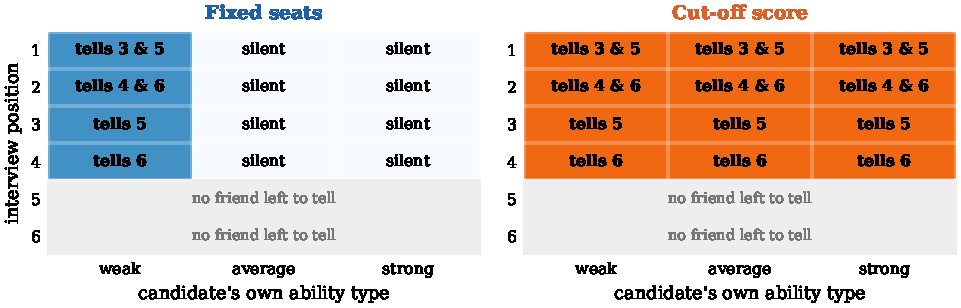
\includegraphics[width=0.66\textwidth]{figures/fig1_who_tells.pdf}
\caption{The equilibrium for two friend groups $\{1,3,5\}$, $\{2,4,6\}$ at friendliness $\alpha=0.2$ (leak model E1). Under either rule it is the only pure equilibrium among 262{,}144 profiles.}\label{fig:who}
\end{figure}
\finding{Under fixed seats only weak candidates tell; under a cut-off everyone does} (Figure~\ref{fig:who}). The pilot's picture survives exhaustive search:
with fixed seats \PilotShareSeats\% of the possible tells are made, with a cut-off \PilotShareBar\%. Under both rules the equilibrium is unique, all 8 best-response runs and all 3
replicator runs end in it, and it remains an exact equilibrium in \PilotBootFracSeats\% (seats) and \PilotBootFracBar\% (cut-off) of \PilotBootRSeats{} bootstrap replicates of the table.

\finding{Why: a weak candidate has almost nothing to lose} (Figure~\ref{fig:why}a,b). Under fixed seats, telling one friend costs a weak candidate \EllSeatsWeak{} percentage points of her own
hiring chance, an average one \EllSeatsAvg{} and a strong one \EllSeatsStrong{} --- a weak candidate is rarely near the last seat, so a boosted friend rarely pushes \emph{her} out.
The friend gains about the same in all three cases (\GainSeatsWeak, \GainSeatsAvg, \GainSeatsStrong{} points). The break-even friendliness $\alpha^\star=(\ell+c)/G$ is therefore
\AstarLocalSeatsWeak, \AstarLocalSeatsAvg{} and \AstarLocalSeatsStrong{} for weak, average and strong candidates (the pilot estimated 0.09, 0.32, 0.37), and the exact equilibria switch at the next grid points:
\AstarGridSeatsWeak, \AstarGridSeatsAvg{} and \AstarGridSeatsStrong. Under a cut-off the loss is exactly zero for every type (Proposition~\ref{prop:bar}) and $\alpha^\star\approx\AstarLocalBarWeak$: any
friendliness above the cost of a message is enough.

\begin{figure}[t]\centering
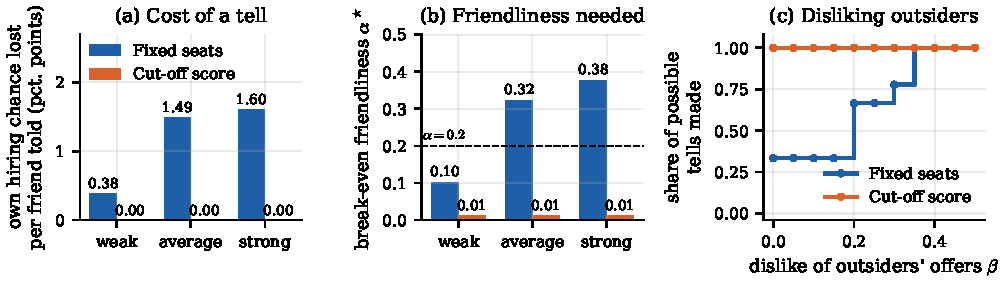
\includegraphics[width=0.92\textwidth]{figures/fig2_why_and_clans.pdf}
\caption{(a) Own hiring chance lost per friend told. (b) Break-even friendliness; types below the dashed line tell at $\alpha=0.2$. (c) Share of possible tells made in equilibrium as candidates
dislike outsiders' offers more ($\alpha=0.2$). Two friend groups, E1.}\label{fig:why}
\end{figure}

\finding{The staircase holds across networks and leak models} (Figure~\ref{fig:alpha}). We solved \XoneCells{} games exactly. Under a cut-off, sharing jumps from nothing to its maximum at the first grid point
above zero in every network. Under fixed seats it climbs in steps --- weak, then average, then strong. A cut-off produces at least as much sharing as fixed seats in \HtwoOk{} of \HtwoCells{}
comparisons, and strictly more in \HtwoStrict; the one exception is discussed below. Three details:
\begin{itemize}
\item \emph{The popular candidate never tells.} In the star network the hub is friends with everyone. Her break-even friendliness is above 1 and she is silent at every $\alpha\le0.5$ under fixed seats, as
Corollary~\ref{cor:hub} says: any seat she hands a friend is taken from herself or from another friend. Sharing in the star therefore stops at 40\% (the two candidates before her).
\item \emph{Everyone friends: nobody tells} under fixed seats (``nobody shares'' passes the deviation test at all \CompGrid{} values of $\alpha$, ``everybody shares'' at \CompSeatsAllShare), and everybody tells under a cut-off
(at \CompBarAllShare{} of the \CompGridPos{} values $\alpha>0$; at the smallest, a few tells are not worth the message cost). This is Proposition~\ref{prop:clique} at $n=6$.
\item \emph{When told questions always come up (E0), a second tell is wasted.} A candidate needs to be told only once, so equilibria differ in \emph{who} tells her, and sharing tops out below 100\%
(4 of 6 tells in two groups). This is the only place we find several equilibria: \XoneMulti{} of \XoneCells{} games, all in \XoneMultiEnvs; the other \XoneUnique{} have exactly one and none has zero.
It is also where the one exception sits (\HtwoViolWhere): fixed seats have \HtwoViolSeatsN{} equilibria sharing \HtwoViolSeatsLo--\HtwoViolSeatsHi\%, the cut-off \HtwoViolBarN{} sharing \HtwoViolBar\%.
\end{itemize}
\finding{How solid are these equilibria?} The reported profile stays an exact equilibrium in at least 95\% of bootstrap replicates in \XoneBootOk{} of \XoneBootTot{} games (\XoneBootOkPct\%). The exceptions sit
on a step of the staircase, where a type is nearly indifferent; even there the 95th-percentile $\varepsilon$ is at most \XoneWorstEpsPP{} percentage points of utility. So the \emph{pattern} is certain and each \emph{threshold} is known to
within one grid step. Uniqueness is a statement about the estimated table, so we also count near-ties: profiles that are within $\varepsilon=0.001$
(one message cost, 0.1 percentage points) of being an equilibrium. The games of Figure~\ref{fig:who} ($\alpha=0.2$) still have exactly
\EpsBneHeadSeats{} (seats) and \EpsBneHeadBar{} (cut-off). Over all \EpsBneGames{} games, \EpsBneMulti{} have more than one: \EpsBneLowAlpha{} at
$\alpha\le0.025$, where a tell is worth about what it costs; \EpsBneEzero{} in E0, where a redundant tell costs exactly $c$; and \EpsBneStep{} on the steps of the
fixed-seats staircase in E1/E2 (up to \EpsBneStepMax{} profiles), where one type is nearly indifferent. Away from these, every cut-off game in E1/E2 has a single
near-equilibrium. Best-response dynamics converged in \XoneBrdOk{} of \XoneBrdTot{} runs, and replicator dynamics ended at an enumerated pure equilibrium in \XoneRepMatch{} of \XoneRepTot{} runs (the other \XoneRepRest{}, all in
the most fragile game, had not settled after 3{,}000 steps). 
\finding{What about mixed and correlated equilibria?} The CCE linear programs bound what any mixed or correlated equilibrium can do. In E1 and E2 the maximum and minimum sharing over \emph{all} CCEs
coincide in \CceSingleEone{} of \CceTotEone{} (E1) and \CceSingleEtwo{} of \CceTotEtwo{} (E2) games, so there no mixed or correlated equilibrium shares more or less than the pure one. E0 is the exception:
the interval is a single point in only \CceSingleEzero{} of \CceTotEzero{} games, and in \CceWiderEzero{} of them it is wider than the range spanned by the pure equilibria (up to \CceMaxWidthEzero{} percentage points wide).
For two friend groups at $\alpha=0.2$ under a cut-off, the \CceExN{} pure equilibria all share \CceExPure\% of the possible tells, while correlated play can share anywhere from \CceExLo\% to \CceExHi\%.
A plausible reason, which we did not test: in E0 a second tell of the same friend is exactly redundant and costs only $c$, so candidates are nearly indifferent about who tells and a CCE can spread redundant tells almost freely.
The pure-equilibrium statements of this section therefore describe E0 less completely than E1 and E2.
Iterated strict dominance (Section~\ref{sec:method}) settles the rest: it solves \DomSolved{} of the \DomTot{} games (pairs \DomPairsSolved/\DomPairsTot, star \DomStarSolved/\DomStarTot, two friend groups \DomTwoGroupsSolved/\DomTwoGroupsTot),
and in each of them the surviving profile is the game's only equilibrium of any kind. All but \DomOpenOutsideEzero{} of the games it leaves open are in E0 (the exception: \DomOpenWhere). On the pairs network, support enumeration finds exactly one mixed
equilibrium in each of the \SuppPairsMixedGames{} games dominance leaves open (E0, fixed seats), next to the two pure ones, with sharing between theirs and inside the CCE interval; since three agents mix there and the root finding is not
exhaustive, there may be more. On the other two networks nothing is claimed about mixed equilibria beyond the CCE bound.

\begin{figure}[t]\centering
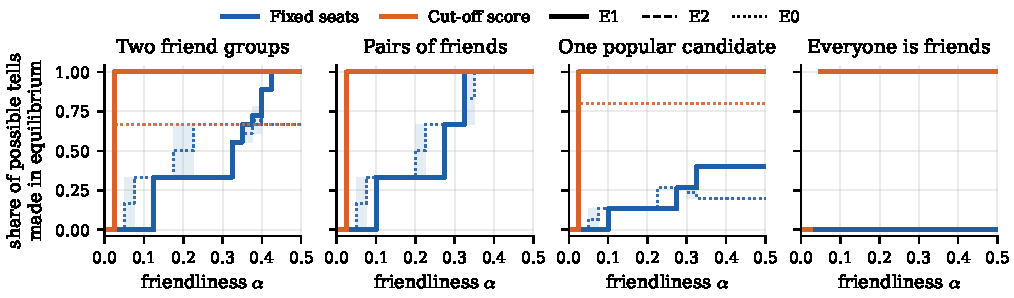
\includegraphics[width=0.93\textwidth]{figures/fig3_sharing_vs_friendliness.pdf}
\caption{Share of possible tells made in equilibrium as candidates care more about friends. Shaded bands: range over multiple equilibria (E0 only). ``Everyone is friends'' shows the profile
that passes the deviation test (E1).}\label{fig:alpha}
\end{figure}

\subsection{What candidates care about (RQ2)}
\begin{table}[t]\centering\small
\caption{Equilibrium sharing for different motives (two friend groups A$=\{1,3,5\}$, B$=\{2,4,6\}$; E1). Every game has exactly one pure equilibrium.
$^\dagger$: exact equilibrium in fewer than 95\% of bootstrap replicates (a type is nearly indifferent).}\label{tab:x2}
\resizebox{0.93\textwidth}{!}{\begin{tabular}{@{}lllrr@{}}
\toprule
What candidates care about & \multicolumn{2}{l}{Who tells, in equilibrium} & \multicolumn{2}{r}{Tells made (\%)} \\
\cmidrule(lr){2-3}\cmidrule(l){4-5}
 & Fixed seats & Cut-off & Seats & Cut-off \\
\midrule
Only own offer (selfish) & nobody & nobody & 0 & 0 \\
Friends' offers too, $\alpha{=}0.2$ & weak & everybody & 33 & 100 \\
\ldots and dislike outsiders, $\beta{=}0.2$ & weak; average$^\dagger$ & everybody & 67 & 100 \\
\ldots and dislike outsiders, $\beta{=}0.4$ & everybody & everybody & 100 & 100 \\
Dislike inequality, $(a,b){=}(0.25,0.1)$ & nobody & nobody & 0 & 0 \\
Dislike inequality, $(a,b){=}(0.5,0.25)$ & nobody & strong (4 of 6 tells)$^\dagger$ & 0 & 22 \\
Dislike inequality, $(a,b){=}(1,0.5)$ & nobody & strong & 0 & 33 \\
Dislike inequality, $(a,b){=}(2,0.5)$ & nobody & nobody & 0 & 0 \\
\midrule
Group A friendly, group B selfish & weak in A & everyone in A & 17 & 50 \\
Only the first interviewees friendly & weak (cand.\ 1--2) & everyone (cand.\ 1--2) & 22 & 67 \\
Only the first interviewees selfish & weak (cand.\ 3--4) & everyone (cand.\ 3--4) & 11 & 33 \\
Group A friendly, group B clannish ($\beta{=}0.3$) & weak; average in B; strong (2 of 6 tells)$^\dagger$ & everybody & 61 & 100 \\
Group A inequality-averse, group B friendly & weak in B & weak in B; average in B; strong (5 of 6 tells) & 17 & 61 \\
\bottomrule
\end{tabular}
}
\end{table}
\finding{Disliking outsiders makes candidates more generous to friends --- but only under fixed seats} (Figure~\ref{fig:why}c). As $\beta$ rises from 0 to 0.5 at fixed $\alpha=0.2$, sharing under
fixed seats rises from \ClanShareMinSeats\% to \ClanShareMaxSeats\% (everyone tells from $\beta=\ClanBetaFull$, i.e.\ $\alpha_{\text{eff}}=\ClanAlphaEffFull$, in line with the strong types' threshold above), and stays at
\ClanShareMinBar\% under a cut-off. This is the Remark of Section~3: with a fixed number of seats, each seat a friend takes is one an outsider loses.

\finding{Fairness-minded candidates behave the other way round} (Table~\ref{tab:x2}). Under fixed seats they never tell. Under a cut-off it is the \emph{strong} who tell, and only for moderate
inequality aversion: a strong candidate expects to be hired and dislikes being ahead of her friends, so she pulls them up; if envy ($a$) is large, the risk of being the one left behind dominates and
telling stops. This is the case Proposition~\ref{prop:bar} excludes, and the only one where behaviour under a cut-off depends on type.

\finding{Motives barely spill over.} In the \MixedGames{} mixed-population games, only \MixedDiffCells{} of \MixedCells{} (candidate, type) choices differs from what that candidate does in a population made entirely of her own kind
(a nearly indifferent strong clannish candidate tells one friend more when the other group is merely friendly). With one friendly and one selfish group, exactly the friendly group shares: weak types under fixed seats, everyone under a cut-off.

\subsection{Can candidates learn it? (RQ3)}
\begin{figure}[t]\centering
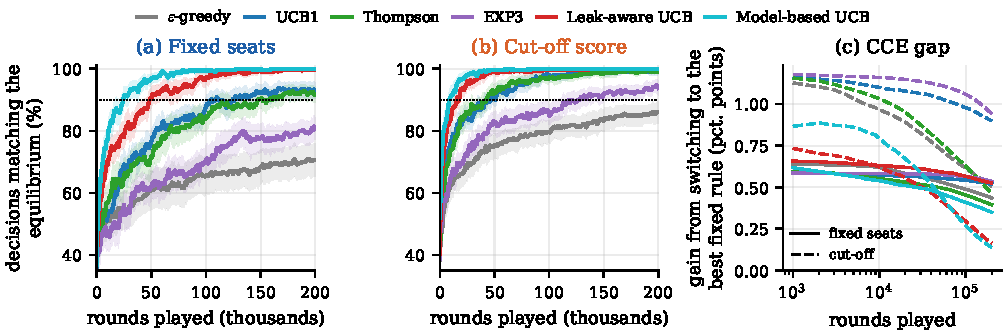
\includegraphics[width=0.93\textwidth]{figures/fig4_learning.pdf}
\caption{Learning in E1, mean over \XthreeSeeds{} seeds with 95\% bootstrap bands. (a,b) Share of the 12 (candidate, type) learners whose best arm is the equilibrium row.
(c) CCE gap of the history of play.}\label{fig:learn}
\end{figure}
\begin{table}[t]\centering\small
\caption{Decisions matching the equilibrium after \XthreeT{} rounds (\%, mean $\pm$ half-width of the 95\% CI over \XthreeSeeds{} seeds; best per column in bold), and median rounds to reach 90\%
(``never ($x$\%)'': the median run did not, $x$\% of runs did), and cumulative regret after \XthreeT{} rounds (Definition~4, in units of one offer, mean over the 12 learners
and \XthreeSeeds{} seeds; lowest in bold). In E0 with a cut-off the equilibria differ only in who makes a redundant tell.}\label{tab:x3}
\resizebox{0.93\textwidth}{!}{\begin{tabular}{@{}lrrrrrrrrrr@{}}
\toprule
 & \multicolumn{2}{c}{E0} & \multicolumn{2}{c}{E1} & \multicolumn{2}{c}{E2} & \multicolumn{2}{c}{Rounds to 90\% (E1)} & \multicolumn{2}{c}{Regret at $T$ (E1)} \\
\cmidrule(lr){2-3}\cmidrule(lr){4-5}\cmidrule(lr){6-7}\cmidrule(lr){8-9}\cmidrule(lr){10-11}
Learner & Seats & Cut-off & Seats & Cut-off & Seats & Cut-off & Seats & Cut-off & Seats & Cut-off \\
\midrule
$\varepsilon$-greedy & 82\,{\scriptsize$\pm$4} & \textbf{74\,{\scriptsize$\pm$3}} & 71\,{\scriptsize$\pm$5} & 86\,{\scriptsize$\pm$3} & 72\,{\scriptsize$\pm$4} & 86\,{\scriptsize$\pm$4} & never\,(20\%) & never\,(50\%) & \textbf{154} & 178 \\
UCB1 & \textbf{96\,{\scriptsize$\pm$2}} & 56\,{\scriptsize$\pm$2} & 93\,{\scriptsize$\pm$3} & 99\,{\scriptsize$\pm$1} & 94\,{\scriptsize$\pm$2} & 99\,{\scriptsize$\pm$1} & 56k & 18k & 246 & 421 \\
Thompson sampling & 93\,{\scriptsize$\pm$2} & 70\,{\scriptsize$\pm$4} & 92\,{\scriptsize$\pm$3} & 99\,{\scriptsize$\pm$1} & 94\,{\scriptsize$\pm$2} & 99\,{\scriptsize$\pm$1} & 78k & 19k & 173 & 191 \\
EXP3 & 93\,{\scriptsize$\pm$2} & 51\,{\scriptsize$\pm$1} & 81\,{\scriptsize$\pm$4} & 94\,{\scriptsize$\pm$2} & 84\,{\scriptsize$\pm$4} & 93\,{\scriptsize$\pm$2} & 141k & 61k & 251 & 442 \\
Leak-aware UCB & \textbf{96\,{\scriptsize$\pm$2}} & 56\,{\scriptsize$\pm$2} & \textbf{100\,{\scriptsize$\pm$0}} & \textbf{100\,{\scriptsize$\pm$0}} & \textbf{100\,{\scriptsize$\pm$0}} & \textbf{100\,{\scriptsize$\pm$0}} & 27k & 7k & 247 & \textbf{70} \\
\bottomrule
\end{tabular}
}
\end{table}
\finding{Yes --- but the signal is tiny, so it takes tens of thousands of interviews.} At equilibrium the best row beats the second-best by only \PayGapMinEoneSeats--\PayGapMaxEoneSeats{} percentage points of utility under
fixed seats and \PayGapMinEoneBar--\PayGapMaxEoneBar{} under a cut-off, while a single outcome is 0 or 1. UCB1 and Thompson sampling nevertheless end with \AgreeUcbEoneSeats\% and \AgreeTsEoneSeats\% (seats)
and \AgreeUcbEoneBar\% and \AgreeTsEoneBar\% (cut-off) of decisions correct in E1 (Table~\ref{tab:x3}); EXP3, which guards against adversarial rewards, and $\varepsilon$-greedy are slower
(\AgreeExpEoneSeats/\AgreeExpEoneBar\% and \AgreeEpsEoneSeats/\AgreeEpsEoneBar\%). Results under E2 are the same within error bars.

\finding{Finding the equilibrium and earning along the way are different things.} Regret ranks the learners almost the other way round (Table~\ref{tab:x3}, last
two columns). Under fixed seats in E1, cumulative regret is \RegretEpsEoneSeats{} for $\varepsilon$-greedy and \RegretTsEoneSeats{} for Thompson sampling, against
\RegretUcbEoneSeats{} for UCB1 and \RegretExpEoneSeats{} for EXP3; under a cut-off \RegretEpsEoneBar{} and \RegretTsEoneBar{} against \RegretUcbEoneBar{} and
\RegretExpEoneBar. So UCB1 ends up with the right answer but pays more to get there, and $\varepsilon$-greedy has the lowest regret under fixed seats
despite the lowest agreement. Plausible reasons, which we did not test: with payoff gaps this small, UCB1's confidence bonus keeps it exploring for a long time,
while $\varepsilon$-greedy's remaining mistakes are on decisions where the wrong row costs little.

\finding{A cut-off is easier to learn than fixed seats} whenever the equilibrium is unique: the gap is larger and the same for all types. In E1 and E2, agreement under a cut-off is at least as high for every learner and significantly higher
(Holm-corrected $p<0.05$) in \BarSeatsSig{} of \BarSeatsTests{} paired tests (the exceptions: \BarSeatsNotSigLearners, at 100\% under both rules). Under fixed seats the slowest learners are the \emph{average} types (UCB1: \TypeUcbEoneSeatsWeak\% of weak, \TypeUcbEoneSeatsAvg\% of average,
\TypeUcbEoneSeatsStrong\% of strong decisions correct), although their gap is not the smallest (\PayGapTypeEoneSeatsWeak, \PayGapTypeEoneSeatsAvg, \PayGapTypeEoneSeatsStrong{} points). A plausible reason, which we did not test: a weak candidate is almost never hired, so her rewards are much less noisy.

\finding{Knowing how leaks work is worth a factor of two to five.} Two learners use it. Leak-aware UCB (UCB1 plus credit for tells that did not land) reaches 90\% agreement in E1 after \TninetyMbEoneSeats{} rounds under fixed seats and
\TninetyMbEoneBar{} under a cut-off, against \TninetyUcbEoneSeats{} and \TninetyUcbEoneBar{} for UCB1. Model-based UCB, which estimates the leak rate and the value of a leaked question and plans with them, needs
\TninetyMuEoneSeats{} and \TninetyMuEoneBar. Both end at 100\% (rounded) in E1 and E2 under both rules. At 20{,}000 rounds Leak-aware UCB is ahead of UCB1 by
$\MbEarlyEoneSeats$ and $\MbEarlyEoneBar$ points (E1) and $\MbEarlyEtwoSeats$ and $\MbEarlyEtwoBar$ points (E2), and Model-based UCB by $\MuEarlyEoneSeats$ and $\MuEarlyEoneBar$ (E1) and $\MuEarlyEtwoSeats$ and
$\MuEarlyEtwoBar$ (E2); all \MbEarlyTests{} and all \MuEarlyTests{} differences are significant after Holm correction. The settled profile of Model-based UCB is an exact equilibrium in \ExactEqMuEoneSeats\% (seats) and
\ExactEqMuEoneBar\% (cut-off) of E1 runs, of Leak-aware UCB in \ExactEqMbEoneSeats\% and \ExactEqMbEoneBar\%, and of UCB1 in \ExactEqUcbEoneSeats\% and \ExactEqUcbEoneBar\%.
The two help in different ways. Against UCB1, the cumulative regret of Leak-aware UCB changes by $\MbRegretEoneBar$ under a cut-off, where the best arm is ``tell everyone'' and each pull also informs every other arm, and by
$\MbRegretEoneSeats$ under fixed seats, where the best arm for most types is silence --- and silence teaches nothing about telling. Model-based UCB lowers regret in all four E1/E2 settings
($\MuRegretEoneSeats$ and $\MuRegretEoneBar$ in E1, $\MuRegretEtwoSeats$ and $\MuRegretEtwoBar$ in E2; significant after Holm correction in \MuRegretSig{} of \MuRegretTests), and it is the only learner that improves on UCB1 in both
regret and agreement under fixed seats ($\varepsilon$-greedy and Thompson sampling also have lower regret there, but lower agreement). A plausible reason, which we did not test: it learns the value of a leaked question from every round in which any arm that tells that friend was played, instead of treating each row of $S$ as a separate arm.
Its leak-rate estimate is used to choose arms, and is right ($\hat p=\MuLeakHatEone$ in E1 and E2, truth $m/Q=0.2$; $\MuLeakHatEzero$ in E0, where every told question comes up). The model is additive across friends, so it cannot
represent a redundant second tell. In E0 under a cut-off, where that matters, its agreement is \AgreeMuEzeroBar\% (UCB1: \AgreeUcbEzeroBar\%) --- see the caution below --- while its regret is still lower ($\MuRegretEzeroBar$).

\finding{Play moves toward the CCE set, but is not yet close to it} (Figure~\ref{fig:learn}c). The CCE gap falls between 10{,}000 and \XthreeT{} rounds for all six learners (to \GapRatioMin--\GapRatioMax{} of its earlier value;
Holm-corrected $p<0.001$ in \GapFallSig{} of \GapFallTests{} tests) and ends at \GapFinalMin--\GapFinalMax{} percentage points. That is about the size of the payoff gaps the learners have to
detect (\PayGapMinEoneSeats--\PayGapMaxEoneSeats{} points under fixed seats), so after \XthreeT{} rounds the history of play is measurably closer to a CCE but not yet near one:
exploration is still being paid for.

\finding{A caution about ``agreement''.} In E0 with a cut-off, agreement looks poor (\AgreeEzeroBarMin--\AgreeEzeroBarMax\%). The game there has \NumEqEzeroBar{} equilibria that differ only in which of two friends tells the last candidate; the learners end up
both telling. The residual gain from deviating is \ExplEzeroBarMin{} percentage points for every learner --- exactly the message cost $c$. They have learned everything that matters and failed only to coordinate on who saves a message.

\subsection{What it costs the company (RQ4)}
\begin{figure}[t]\centering
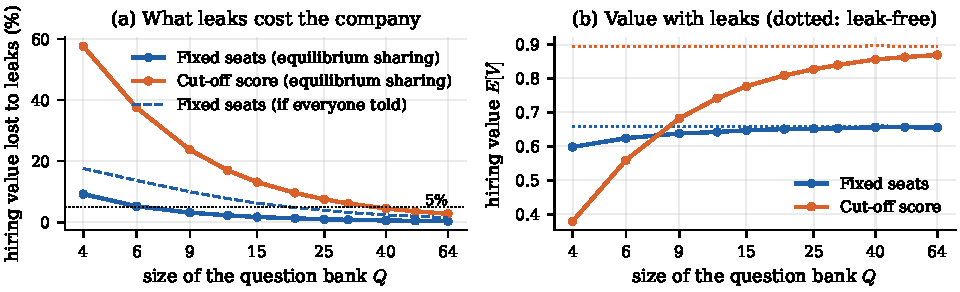
\includegraphics[width=0.78\textwidth]{figures/fig5_company_loss.pdf}
\caption{Company's hiring value under equilibrium sharing as the question bank grows (E2, $\alpha=0.2$, $m=3$ questions per interview). 95\% block-bootstrap intervals (\XfourBoot{} replicates) are narrower than the markers.}\label{fig:company}
\end{figure}
\finding{At $\alpha=0.2$, leaks hurt a cut-off company about ten times more --- mostly because more people tell.} With the pilot's bank of 15 questions, equilibrium sharing costs \LamSeatsQFifteen\% of hiring value under fixed seats and \LamBarQFifteen\% under a cut-off;
across all bank sizes the cut-off loses \LamRatioMin--\LamRatioMax{} times more, and the bootstrap intervals are disjoint at all \LamOrderTot{} sizes (Figure~\ref{fig:company}a).
To keep the loss below 5\% the company needs $Q\ge\QFiveSeats$ under fixed seats and $Q\ge\QFiveBar$ under a cut-off. Proposition~\ref{prop:leak} explains the shape: the leaked fraction falls like $m\,n_j/Q$.
Two effects add up, and they are not equally large. The first is \emph{who} tells: at $\alpha=0.2$, \XfourShareBar\% of possible tells are made under a cut-off and \XfourShareSeats\% under fixed seats.
The second is the rule itself: every leaked mark can lift someone over a fixed line, whereas under fixed seats a leak only reorders candidates. The dashed line in Figure~\ref{fig:company}a separates them.
If everyone told under both rules, fixed seats would lose \LamAllSeatsQFifteen\% at $Q=15$ (against \LamAllBarQFifteen\%), the cut-off would lose only \LamAllRatioMin--\LamAllRatioMax{} times more,
and fixed seats would need $Q\ge\QFiveAllSeats$ rather than \QFiveSeats. The tenfold gap is therefore specific to a friendliness at which only weak candidates tell under fixed seats;
wherever candidates are friendly enough that everyone tells under both rules, the everyone-tells comparison is the relevant one.

\finding{But the cut-off is still the better rule once the bank is large enough} (Figure~\ref{fig:company}b). Without leaks a cut-off hires better (value \VNoLeakBar{} against \VNoLeakSeats): it can hire three good
candidates or none, where fixed seats must always hire two. Leaks eat this advantage only for small banks: fixed seats give more value up to $Q=\CrossQBarWorseUpTo$, the cut-off from $Q=\CrossQBarBetterFrom$
(\VEqBarQFifteen{} against \VEqSeatsQFifteen{} at $Q=15$). For a company the message is not ``avoid cut-offs'' but ``a cut-off needs a question bank several times larger''.

\subsection{Verdict on the hypotheses, deviations and limits}
\begin{table}[t]\centering\small
\caption{The five hypotheses fixed in the project review, the refutation criterion fixed with them, and what the experiments say.}\label{tab:hyp}
\begin{tabular}{@{}p{0.5cm}>{\raggedright\arraybackslash}p{4.1cm}>{\raggedright\arraybackslash}p{3.3cm}>{\raggedright\arraybackslash}p{6.1cm}>{\raggedright\arraybackslash}p{2.0cm}@{}}
\toprule
 & Hypothesis & Refuted if (review) & Evidence & Verdict\\\midrule
H1 & Under fixed seats, $\alpha^\star$ is highest for the types most likely to be pivotal & $\alpha^\star$ flat, or lowest for pivotal types &
$\alpha^\star=\AstarLocalSeatsWeak<\AstarLocalSeatsAvg<\AstarLocalSeatsStrong$, in the order of the chance that a tell costs one's own seat ($\ell=\EllSeatsWeak,\EllSeatsAvg,\EllSeatsStrong$ points) & Supported\\
H2 & Cut-off shares more than fixed seats for every $\alpha\in[0,0.5]$ & Fixed seats share more at some $\alpha$ &
Holds in all \HtwoCellsNoEzero{} E1/E2 comparisons. In E0 fails once (\HtwoViolWhere): fixed seats have equilibria sharing up to \HtwoViolSeatsHi\%, the cut-off \HtwoViolBar\% &
Refuted once (E0); holds in E1/E2\\
H3 & Fixed seats: sharing rises with $\beta$; cut-off: no effect & No rise under fixed seats, or an effect under a cut-off & \ClanShareMinSeats\%$\to$\ClanShareMaxSeats\% (never falling) vs.\ constant \ClanShareMinBar\% & Supported\\
H4 & No-regret play nears the CCE set; model-based learners are faster & CCE gap does not fall, or not faster &
CCE gap falls for \GapFallSig{} of \GapFallTests{} learners but ends at \GapFinalMin--\GapFinalMax{} points, the size of the payoff gaps; Model-based UCB reaches 90\% in \TninetyMuEoneSeats/\TninetyMuEoneBar{} rounds (leak-aware UCB: \TninetyMbEoneSeats/\TninetyMbEoneBar) vs.\ \TninetyUcbEoneSeats/\TninetyUcbEoneBar{} for UCB1 & Faster: supported; nears the CCE set: weak$^\ast$\\
H5 & $\Lambda_{\textsc{bar}}>\Lambda_{\textsc{seats}}$, and fixed seats need a smaller $Q$ for $\Lambda<5\%$ & CI includes 0, or order reversed &
At $\alpha=0.2$: \LamRatioMin--\LamRatioMax$\times$ larger, disjoint CIs at every $Q$; $Q\ge\QFiveSeats$ vs.\ $Q\ge\QFiveBar$. If everyone told: \LamAllRatioMin--\LamAllRatioMax$\times$; $Q\ge\QFiveAllSeats$ vs.\ $Q\ge\QFiveAllBar$ & Supported\\
\bottomrule
\end{tabular}

\raggedright\footnotesize $^\ast$ The CCE gap falls but is not yet small. The model-based learner is a reduced-form version of the one in the review (it estimates the value $\beta$ of a leaked question, not $\Delta$, and plans alone rather than best-responding in an estimated game of all candidates); the leak-aware learner is only UCB1 with credit for tells that did not land (Section~\ref{sec:method}) and has lower regret only under a cut-off.
\end{table}
Judged by the refutation criteria fixed in the review (Table~\ref{tab:hyp}), H1, H3 and H5 are supported. H4 is not refuted, with unequal support: the faster-learner half holds clearly (for a reduced-form model-based learner and for the simpler leak-aware one), but the CCE gap falls without
becoming small. H2 is refuted at one point: in E0, where the game has several equilibria, some fixed-seats equilibria share more
than the cut-off's; in E1 and E2 it holds in every comparison. \textbf{Deviations from the review plan:}
(i)~tables use 2{,}000 days per cell, not the pilot's 8{,}000; precision is instead reported per equilibrium by the bootstrap;
(ii)~the ``model-based'' learner of the review is built in two simpler forms: Leak-aware UCB (UCB1 with counterfactual credit; its leak-rate estimate is logged but not used) and Model-based UCB (a reduced-form model of leaked questions, planned with by one candidate alone); both need the friend to report how many told questions came up;
(iii)~mixed equilibria were sought by replicator dynamics, by iterated dominance on all networks and by support enumeration on the pairs network only (agents have four or eight actions on the other two),
with the CCE programs bounding what remains;
(iv)~the CCE programs use a coarser grid ($\alpha$ in steps of 0.05) for two friend groups; (v)~the complete network at $n=6$ was handled by deviation tests, and $n=8$ was not attempted.
\textbf{Limits.} Types are coarse and rounds are independent: there is no reputation, and placed candidates do not leave the pool (a stochastic game~\cite{shapley}). Networks are fixed and small.
There is no real leak data, so every claim is comparative (seats vs.\ cut-off, weak vs.\ strong), not a prediction of how much real candidates share.
The bootstrap measures Monte Carlo error, not sensitivity to $\Delta$, $\sigma$ or $K/n$, which we held fixed.

% =====================================================================================================
\section{Contribution}
{\centering\footnotesize
\begin{tabular}{@{}p{2.5cm}>{\raggedright\arraybackslash}p{5.3cm}>{\raggedright\arraybackslash}p{6.3cm}>{\raggedright\arraybackslash}p{2.3cm}@{}}
\toprule
Member & Task assigned in the review & Where it is delivered & Status\\\midrule
Jash Bharat Pasad & Formulation, proofs; utility types (X2); company analysis (X4); writing, integration &
Sections 2--3, Corollary~1; \texttt{utility.py}, \texttt{run\_x2.py}, \texttt{run\_x4.py}; Table~\ref{tab:x2}, Figure~\ref{fig:company}; report & Fulfilled\\
Bhavay Goyal & Simulator (E0--E2, networks), payoff tables, verification checks, pipeline &
\texttt{config.py}, \texttt{env.py}, \texttt{tables.py}, \texttt{checks.py}, unit tests; Table~\ref{tab:checks} & Fulfilled\\
Chaitanya Bhoite & Level-1 solvers (BNE, mixed equilibria, CCE program, bootstrap $\varepsilon$); X1 &
\texttt{game.py}, \texttt{solvers.py}, \texttt{support\_enum.py}, \texttt{analysis.py}, \texttt{run\_x1.py}, \texttt{run\_cce.py}, \texttt{run\_support.py}; Figures~\ref{fig:who}--\ref{fig:alpha} & Fulfilled; support enumeration on the pairs network only\\
Vishnu Sinha & Level-2 learners (incl.\ model-based); regret and CCE metrics; X3; statistics &
\texttt{learners.py}, \texttt{learning.py}, \texttt{stats.py}, \texttt{run\_x3.py}; Figure~\ref{fig:learn}, Table~\ref{tab:x3} & Fulfilled; model-based learner in reduced form\\
\bottomrule
\end{tabular}\par}
\vspace{3pt}
Core (verified simulator, X1--X3, H1--H4) and target (X4, H5) deliverables are complete; the stretch target $n=8$ is not.
Every number above is generated from the result files in the repository by \texttt{experiments/make\_figures.py}.

{\footnotesize\setlength{\columnsep}{14pt}
\begin{multicols}{2}
\begin{thebibliography}{15}\setlength{\itemsep}{0pt}\setlength{\parskip}{0pt}
\bibitem{blind} Team Blind. Candidate confessed to memorizing leaked interview questions. \url{https://www.teamblind.com}, accessed Sept.\ 2026.
\bibitem{glider} Glider AI. Leaked interview questions: How candidates get answers. \url{https://glider.ai}, accessed Sept.\ 2026.
\bibitem{lazear} E.~P. Lazear and S. Rosen. Rank-order tournaments as optimum labor contracts. \emph{J. Polit. Econ.}, 89(5):841--864, 1981.
\bibitem{krakel} M. Kr\"akel. Helping and sabotaging in tournaments. \emph{Int. Game Theory Rev.}, 7(2):211--228, 2005.
\bibitem{li} Y. Li and V. Conitzer. Game-theoretic question selection for tests. \emph{J. Artif. Intell. Res.}, 59:437--462, 2017.
\bibitem{ucb} P. Auer, N. Cesa-Bianchi, and P. Fischer. Finite-time analysis of the multiarmed bandit problem. \emph{Machine Learning}, 47:235--256, 2002.
\bibitem{exp3} P. Auer, N. Cesa-Bianchi, Y. Freund, and R.~E. Schapire. The nonstochastic multiarmed bandit problem. \emph{SIAM J. Comput.}, 32(1):48--77, 2002.
\bibitem{thompson} W.~R. Thompson. On the likelihood that one unknown probability exceeds another in view of the evidence of two samples. \emph{Biometrika}, 25(3/4):285--294, 1933.
\bibitem{hart} S. Hart and A. Mas-Colell. A simple adaptive procedure leading to correlated equilibrium. \emph{Econometrica}, 68(5):1127--1150, 2000.
\bibitem{wellman} M.~P. Wellman. Methods for empirical game-theoretic analysis. In \emph{Proc. AAAI}, pages 1552--1556, 2006.
\bibitem{shoham} Y. Shoham and K. Leyton-Brown. \emph{Multiagent Systems: Algorithmic, Game-Theoretic, and Logical Foundations}. Cambridge University Press, 2008.
\bibitem{fehr} E. Fehr and K.~M. Schmidt. A theory of fairness, competition, and cooperation. \emph{Q. J. Econ.}, 114(3):817--868, 1999.
\bibitem{holm} S. Holm. A simple sequentially rejective multiple test procedure. \emph{Scand. J. Stat.}, 6(2):65--70, 1979.
\bibitem{shapley} L.~S. Shapley. Stochastic games. \emph{Proc. Natl. Acad. Sci.}, 39(10):1095--1100, 1953.
\end{thebibliography}
\end{multicols}}
\end{document}
